%
% This work is licensed under a Creative Commons Attribution-ShareAlike 4.0 International License.
% http://creativecommons.org/licenses/by-sa/4.0/
%
\documentclass{beamer}
\usetheme[pageofpages=of,% String used between the current page and the
                         % total page count.
          bullet=circle,% Use circles instead of squares for bullets.
          titleline=true,% Show a line below the frame title.
          alternativetitlepage=true,% Use the fancy title page.
	  titlepagelogo=images/logoM-circl-Forensics.png,% Logo for the first page.
%          watermark=watermark-polito,% Watermark used in every page.
%          watermarkheight=100px,% Height of the watermark.
%          watermarkheightmult=4,% The watermark image is 4 times bigger
                                % than watermarkheight.
          ]{Torino}

\usepackage[utf8]{inputenc}
\usepackage{listings}
\usepackage{color}
\usepackage[font=small,labelfont=bf]{caption}
\usepackage{transparent}
\usepackage{siunitx}

\usepackage[norndcorners,customcolors]{hf-tikz}
\hfsetbordercolor{yellow}
\hfsetfillcolor{yellow}

\lstset{ 
  backgroundcolor=\color{white},   % choose the background color; you must add \usepackage{color} or \usepackage{xcolor}
  basicstyle=\footnotesize,        % the size of the fonts that are used for the code
  breakatwhitespace=false,
}


\author{CIRCL \emph{TLP:CLEAR}}
\title{CIRCL - Digital Forensics 1.0.3}
\subtitle{Introduction: Windows-, Memory- and File Forensics}
\institute{info@circl.lu}
\date{December, 2024}



\begin{document}
\begin{frame}[t,plain]
\titlepage
\end{frame}

\begin{frame}
  \frametitle{Overview}
  \begin{itemize}
  \item[]
      \begin{enumerate}
%          \setcounter{enumi}{10}
          \item Windows Registry
          \item Event Logs
          \item Other Sources of Information
          \item Malware Analysis
          \item Analysing files
          \item Live Response
          \item Memory Forensics
          \item Bibliography and Outlook
      \end{enumerate}

  \end{itemize}
\end{frame}


%
% This work is licensed under a Creative Commons Attribution-ShareAlike 4.0 International License.
% http://creativecommons.org/licenses/by-sa/4.0/
%

% DO NOT COMPILE THIS FILE DIRECTLY!
% This is included by the other .tex files.


\begin{frame}
    \includegraphics[scale=.3]{images/logo-circl-Forensics.png}
    \begin{itemize}
        \item[]
        \item[]
        \item[] 1. Windows Registry
    \end{itemize}
\end{frame}


\begin{frame}[fragile]
  \frametitle{1.1 About: Windows Registry}
    \begin{itemize}
        \item MS DOS and old Windows
            \begin{itemize}
                \item On system boot: What programs to load
                \item How the system interact with the user
                \begin{itemize}
			\item[] $\to$ \texttt{autoexec.bat}
			\item[] $\to$ \texttt{config.sys}
			\item[] $\to$ \texttt{system.ini}
			\item[] $\to$ \texttt{win.ini}
                \end{itemize}
            \end{itemize}
        \item \url{https://support.microsoft.com/en-us/help/256986/}
            \begin{itemize}
                \item A central hierarchical database
                \item Replace text based config files
                \item Contains information for operating
                \begin{itemize}
                    \item Hardware system wide
                    \item OS all aspects
                    \item Applications installed
                    \item User preferences / behavior
                \end{itemize}
            \end{itemize}
    \item[] $\to$ A gold mine for forensics
    \end{itemize}
\end{frame}


\begin{frame}[fragile]
  \frametitle{1.1 About: Windows Registry}
    \begin{figure}
        \includegraphics[scale=0.43]{images/nomenclature.pdf}
        \captionsetup{labelformat=empty,labelsep=none}
        \transparent{0.9}%
        \caption[]{\tiny Key data structures contains a last write time stamp}
    \end{figure}
\end{frame}


\begin{frame}[fragile]
  \frametitle{1.1 About: Windows Registry}
    \begin{itemize}
        \item Hive files: Location
            \begin{itemize}
                \item[] \begin{verbatim}%SystemRoot%\system32\config\end{verbatim}
                \item[] $\to$ \texttt{SAM, SECURITY, SYSTEM, SOFTWARE}
                \item[] \begin{verbatim}%UserProfile%\NTUSER.DAT\end{verbatim}
                \item[] \begin{verbatim}%UserProfile%\AppData\Local\Microsoft\Windows\UsrClass.dat\end{verbatim}
            \end{itemize}
        \item[] $\to$ Created during system boot
	\item[]
        \item How often do you manually edit the Registry?
            \begin{itemize}
		\item \texttt{regedit.exe}
                \item Black Magic for many admins
		\item[] $\to$ Every user interacts with the Registry
            \end{itemize}
	\item[]
        \item Timestamps $\to$ Timeline
    \end{itemize}
\end{frame}


\begin{frame}[fragile]
  \frametitle{1.2 Under the hood: Key Cell}
  \definecolor{light-gray}{gray}{0.70}
  \begin{lstlisting}[basicstyle=\tiny,escapechar=§]
     0000:  §\colorbox{light-gray}{a0ff ffff}§ 6e6b 2000  6f0f 0e3b b78d d101  ....nk .o..;....
     0010:  0200 0000 085e 0500  0000 0000 0000 0000  .....^..........
     0020:  ffff ffff ffff ffff  0200 0000 0021 0500  .............!..
     0030:  102e 0000 ffff ffff  0000 0000 0000 0000  ................
     0040:  1400 0000 1000 0000  0000 0000 0a00 0000  ................
     0050:  496e 7465 7266 6163  6573 0080 0200 0000  Interfaces......
  \end{lstlisting}
  \begin{lstlisting}[basicstyle=\tiny]
 Offsets:    0x00       0       4        Size
             0x04       4       2        Node ID
             0x06       6       2        Node type
             0x08       8       8        Last write time
                  ...      ...
             0x4c      76       2        Lenght of key name
             0x50      80     <76>       key name + padding
  \end{lstlisting}
  \begin{itemize}
      \item Exercise: Calculate the size of the key cell
      \begin{itemize}
          \item[] \texttt{a0 ff ff ff}
          \item[]
      \end{itemize}
      \item Exercise: Calculate the size of the key name
      \begin{itemize}
          \item[] \texttt{0a 00}
      \end{itemize}
  \end{itemize}
\end{frame}


\begin{frame}[fragile]
  \frametitle{1.2 Under the hood: Value Cell}
  \definecolor{light-gray}{gray}{0.70}
  \begin{lstlisting}[basicstyle=\tiny,escapechar=§]
     0000:                        §\colorbox{light-gray}{d8ff ffff}§ 766b 0d00          ....vk..
     0010:  0400 0080 0200 0000  0400 0000 0100 0000  ................
     0020:  4c61 7374 4b6e 6f77  6e47 6f6f 6400 0000  LastKnownGood...
  \end{lstlisting}
  \begin{lstlisting}[basicstyle=\tiny]
 Offset:     0x00       0       4        Size
             0x04       4       2        Node ID
             0x06       6       2        Value name length
             0x08       8       4        Data lenght
             0x0c      12       4        Data offset
             0x10      16       4        value typw
  \end{lstlisting}
  \begin{itemize}
      \item Exercise: Calculate the size of the value cell
      \begin{itemize}
          \item[] \texttt{d8 ff ff ff}
          \item[]
      \end{itemize}
      \item Exercise: Calculate the size of the value name length
      \begin{itemize}
          \item[] \texttt{0d 00}
      \end{itemize}
  \end{itemize}
\end{frame}


\begin{frame}[fragile]
  \frametitle{1.3 Hive files}
   \begin{itemize}
       \item[]
   \begin{itemize}
      \item SAM
      \begin{itemize}
          \item Security Accounts Manager: Local users
      \end{itemize}
      \item Security
      \begin{itemize}
          \item Audit settings
          \item Machine, domain SID
      \end{itemize}
      \item System
      \begin{itemize}
          \item Hardware configuration
          \item System configuration
       \end{itemize}
      \item Software
      \begin{itemize}
          \item Windows settings
          \item Application information
      \end{itemize}
      \item NTUser.dat
      \begin{itemize}
          \item User behavior and settings
      \end{itemize}
      \item UsrClass.dat
      \begin{itemize}
          \item Graphical User Interface information
      \end{itemize}
   \end{itemize}
   \end{itemize}
\end{frame}


\begin{frame}[fragile]
  \frametitle{1.3 Hive files}
    \begin{itemize}
        \item Windows XP:
        \item[] \begin{verbatim}C:\Documents and Settings\<username>\NTUSER.DAT\end{verbatim}
        \item[] \begin{verbatim}C:\Documents and Settings\<username>\Local Settings\\end{verbatim}
        \item[] \begin{verbatim}   Application Data\Microsoft\Windows\UsrClass.dat\end{verbatim}
        \item[]
        \item Windows Vista and above:
        \item[] \begin{verbatim}C:\Users\<user>\NTUSER.DAT\end{verbatim}
        \item[] \begin{verbatim}C:\Users\<user>\AppData\Local\Microsoft\Windows\\end{verbatim}
        \item[] \begin{verbatim}   UsrClass.dat\end{verbatim}
        \item[]
	\item \begin{verbatim}C:\Windows\inf\setupapi.log\end{verbatim} (Plug and Play Log)
    \end{itemize}
\end{frame}






\begin{frame}[fragile]
  \frametitle{1.3 Hive files - Exercise: Get hive files}
    \begin{lstlisting}[basicstyle=\tiny]
Extract registry hive files from forensic image
===============================================
























_
      mkdir registry/out
    \end{lstlisting}
\end{frame}


\begin{frame}[fragile]
  \frametitle{1.3 Hive files - Exercise: Get hive files}
    \begin{lstlisting}[basicstyle=\tiny]
Extract registry hive files from forensic image
===============================================

   1. Investigate Meta-Information
   -------------------------------
      ewfinfo image.E01
      ewfexport image.E01



















_
      mkdir registry/out
    \end{lstlisting}
\end{frame}


\begin{frame}[fragile]
  \frametitle{1.3 Hive files - Exercise: Get hive files}
    \begin{lstlisting}[basicstyle=\tiny]
Extract registry hive files from forensic image
===============================================

   1. Investigate Meta-Information
   -------------------------------
      ewfinfo image.E01
      ewfexport image.E01


   2. Mount evidences
   ------------------
      sudo mkdir /media/case1
      mmls image.raw
      sudo mount -o ro,offset=$((512*63)) image.raw /media/case1/













_
    \end{lstlisting}
\end{frame}


\begin{frame}[fragile]
  \frametitle{1.3 Hive files - Exercise: Get hive files}
    \begin{lstlisting}[basicstyle=\tiny]
Extract registry hive files from forensic image
===============================================

   1. Investigate Meta-Information
   -------------------------------
      ewfinfo image.E01
      ewfexport image.E01


   2. Mount evidences
   ------------------
      sudo mkdir /media/case1
      mmls image.raw
      sudo mount -o ro,offset=$((512*63)) image.raw /media/case1/


   3. Copy files
   -------------
      mkdir registry
      cp /media/case1/WINDOWS/system32/config/SAM registry
      cp /media/case1/WINDOWS/system32/config/software registry
      cp /media/case1/WINDOWS/system32/config/system registry
      cp /media/case1/WINDOWS/system32/config/SECURITY registry
      cp /media/case1/Documents\ and\ Settings/Jean/NTUSER.DAT registry
      cp /media/case1//Documents\ and\ Settings/Jean/Local\ Settings/
         Application\ Data/Microsoft/Windows/UsrClass.dat registry/
      ls registry/
      mkdir registry/out
    \end{lstlisting}
\end{frame}


\begin{frame}[fragile]
  \frametitle{1.4 RegRipper}
  \begin{itemize}
	  \item \url{https://github.com/keydet89/RegRipper4.0}
	  \item Plugins: ~385
  \end{itemize}
    \begin{lstlisting}[basicstyle=\tiny]
regripper -h
	Rip v.3.0 - CLI RegRipper tool	
	Rip [-r Reg hive file] [-f profile] [-p plugin] [options]
	Parse Windows Registry files, using either a single module, or a profile.


ls /usr/lib/regripper/plugins | grep pl$ | wc -l
	249


ls /usr/lib/regripper/plugins | grep -v pl$
	all
	amcache
	ntuser
	sam
	security
	software
	syscache
	system
	usrclass
    \end{lstlisting}
\end{frame}


\begin{frame}[fragile]
  \frametitle{1.4 RegRipper - Examples}
  \begin{lstlisting}[basicstyle=\tiny]
     regripper -p compname -r software 
	Select not found.


     regripper -p compname -r system 
	ComputerName    = JEAN-13FBF038A3
	TCP/IP Hostname = jean-13fbf038a3


     regripper -p run -r NTUSER.DAT 

	Software\Microsoft\Windows\CurrentVersion\Run
	LastWrite Time 2008-07-18 04:36:52Z
	  MSMSGS - "C:\Program Files\Messenger\msmsgs.exe" /background
	  Aim6 - "C:\Program Files\AIM6\aim6.exe" /d locale=en-US ee://aol/imApp


     regripper -p run -r software 

	Microsoft\Windows\CurrentVersion\Run
	LastWrite Time 2008-07-06 07:21:46Z
	  VMware User Process - C:\Program Files\VMware\VMware Tools\VMwareUser.exe
	  VMware Tools - C:\Program Files\VMware\VMware Tools\VMwareTray.exe

	Microsoft\Windows\CurrentVersion\Run\OptionalComponents
	LastWrite Time 2008-07-06 07:21:46Z
  \end{lstlisting}
\end{frame}


\begin{frame}[fragile]
  \frametitle{1.4 RegRipper - Examples}
  \begin{lstlisting}[basicstyle=\tiny]
   mkdir registry/out

   regripper -f sam -r SAM > out/sam.txt
   regripper -a     -r SAM > out/sam2.txt
   less registry/out/sam.txt

	User Information
	-------------------------
	Username        : Administrator [500]
	Full Name       : 
	User Comment    : Built-in account for administering the computer/domain
	Account Type    : Default Admin User
	Account Created : 2008-05-13 22:20:14Z
	Name            :  
	Last Login Date : 2008-07-21 01:22:18Z
	Pwd Reset Date  : 2008-05-13 22:23:39Z
	Pwd Fail Date   : Never
	Login Count     : 24
	Embedded RID    : 500
	  --> Password does not expire
	  --> Normal user account

	Username        : Guest [501]
	Full Name       : 
	User Comment    : Built-in account for guest access to the computer/domain
	Account Type    : Default Guest Acct
	Account Created : 2008-05-13 22:20:14Z
  \end{lstlisting}
\end{frame}


\begin{frame}[fragile]
  \frametitle{1.5 RegRipper: Exercise}
  \begin{enumerate}
      \item Extract Hive files from invected PC
      \item Rip them with RegRipper profiles
      \item Collect important general information
      \item Try to find incident related artefacts
      \item Add the information to report
  \end{enumerate}
  \begin{lstlisting}[basicstyle=\tiny]















_
  \end{lstlisting}
\end{frame}


\begin{frame}[fragile]
  \frametitle{1.5 RegRipper: Exercise}
  \begin{enumerate}
      \item Extract Hive files from invected PC
      \item Rip them with RegRipper profiles
      \item Collect important general information
      \item Try to find incident related artefacts
      \item Add the information to report
  \end{enumerate}
  \begin{lstlisting}[basicstyle=\tiny]
mkdir registry/out

     regripper -a -r SAM          > out/sam.txt
     regripper -a -r SECURITY     > out/security.txt
     regripper -a -r software     > out/software.txt
     regripper -a -r system       > out/system.txt
     regripper -a -r NTUSER.DAT   > out/NTUser.txt
     regripper -a -r UsrClass.dat > out/UsrClass.txt

     ls -lh out/
	  24K Nov 11 07:46 NTUser.txt
         7.1K Nov 11 07:47 sam.txt
          603 Nov 11 07:46 security.txt
         658K Nov 11 07:46 software.txt
         157K Nov 11 07:46 system.txt
         1.5K Nov 11 07:47 UsrClass.txt
  \end{lstlisting}
\end{frame}


\begin{frame}[fragile]
  \frametitle{1.6 General information: sam, security}
  \begin{lstlisting}[basicstyle=\tiny]
    less out/SAM.txt

	Username        : Administrator [500]
		Last Login Date : 2008-07-21 01:22:18Z
		Pwd Fail Date   : Never
		Login Count     : 24

	Username        : Jean [1004]
		Last Login Date : 2008-07-20 00:00:41Z
		Pwd Fail Date   : Never
		Login Count     : 80

	Group Name    : Administrators [7]
	LastWrite     : 2008-05-14 05:35:35Z
	  S-1-5-21-484763869-796845957-839522115-1006
	  S-1-5-21-484763869-796845957-839522115-1008
	  S-1-5-21-484763869-796845957-839522115-1007
	  S-1-5-21-484763869-796845957-839522115-1005
	  S-1-5-21-484763869-796845957-839522115-1003
	  S-1-5-21-484763869-796845957-839522115-500
	  S-1-5-21-484763869-796845957-839522115-1004


    less out/security.txt
	
  \end{lstlisting}
\end{frame}


\begin{frame}[fragile]
  \frametitle{1.6 General information: system, software}
  \begin{lstlisting}[basicstyle=\tiny]
    regripper -p winver -r software 

	ProductName               Microsoft Windows XP
	CSDVersion                Service Pack 3      
	BuildLab                  2600.xpsp.080413-2111
	RegisteredOrganization                        
	RegisteredOwner           Jean User           
	InstallDate               2008-05-13 21:29:32Z


    regripper -p networkcards -r software 

	Description                                Key LastWrite time                                
	VMware Accelerated AMD PCNet Adapter       2008-05-14 05:31:26Z


    regripper -p uninstall -r software

	2008-07-19 23:32:23Z
	  VMware Tools v.3.2.0.1288
	.....


    regripper -p ips -r system

	IPAddress            Domain
	192.168.117.129      localdomain   
  \end{lstlisting}
\end{frame}


\begin{frame}[fragile]
  \frametitle{1.6 General information: system, software}
  \begin{lstlisting}[basicstyle=\tiny]
    regripper -p profilelist -r software

	Path      : %SystemDrive%\Documents and Settings\Jean
	SID       : S-1-5-21-484763869-796845957-839522115-1004
	LastWrite : 2008-07-21 01:18:00Z

	Path      : %SystemDrive%\Documents and Settings\Devon
	SID       : S-1-5-21-484763869-796845957-839522115-1007
	LastWrite : 2008-07-12 06:04:40Z

	Path      : %SystemDrive%\Documents and Settings\Administrator
	SID       : S-1-5-21-484763869-796845957-839522115-500
	LastWrite : 2008-07-21 01:31:01Z


    regripper -p shutdown -r system 

	ControlSet001\Control\Windows key, ShutdownTime value
	LastWrite time: 2008-07-21 01:31:32Z
	ShutdownTime  : 2008-07-21 01:31:32Z


    regripper -p timezone -r system

	ControlSet001\Control\TimeZoneInformation
	LastWrite Time 2008-05-14 06:55:57Z
	  DaylightName   -> GMT Daylight Time
  \end{lstlisting}
\end{frame}


\begin{frame}[fragile]
  \frametitle{1.7 Tracing user activity}
  \begin{enumerate}
	  \item[] MRU - Most Recently Used
      \begin{enumerate}
	      \item[] Open/Save As dialog box
              \begin{lstlisting}[basicstyle=\tiny]
  regripper -p comdlg32 -r NTUSER.DAT
              \end{lstlisting}
	      \item[] Recent Docs opened via Win. Explorer
		      \begin{lstlisting}[basicstyle=\tiny]
  regripper -p recentdocs -r NTUSER.DAT
              \end{lstlisting}
      \end{enumerate}
	  \item[] ShellBags (Win7+)
      \begin{enumerate}
	      \item[] Properties of folders
              \begin{lstlisting}[basicstyle=\tiny]
  regripper -p shellbags -r UsrClass.dat
              \end{lstlisting}
      \end{enumerate}
	  \item[] Program execution
      \begin{enumerate}
	      \item[] UserAssist: GUI based launched
              \begin{lstlisting}[basicstyle=\tiny]
  regripper -p userassist -r NTUSER.DAT
              \end{lstlisting}
	      \item[] ShimCache: Track compatibility issues
              \begin{lstlisting}[basicstyle=\tiny]
  regripper -p shimcache -r system
              \end{lstlisting}
      \end{enumerate}
  \end{enumerate}
\end{frame}


\begin{frame}[fragile]
  \frametitle{1.7 Tracing user activity}
  \begin{enumerate}
	  \item[] USB attached devices
      \begin{enumerate}
	      \item[] USBStor: Attached devices
              \begin{lstlisting}[basicstyle=\tiny]
  less /media/case1/WINDOWS/setupapi.log
  regripper -p usbstor -r system
              \end{lstlisting}
              \item[] USBStor: Vendor \& Product ID
              \begin{lstlisting}[basicstyle=\tiny]
  regripper -p usb -r system
              \end{lstlisting}
              \item[] MountedDevices
              \begin{lstlisting}[basicstyle=\tiny]
  regripper -p mountdev -r system
              \end{lstlisting}
              \item[] MountPoints
              \begin{lstlisting}[basicstyle=\tiny]
  regripper -p mp2 -r NTUSER.DAT
              \end{lstlisting}
      \end{enumerate}
	  \item[] 
	  \item[] SANS Posters:
          \begin{enumerate}
	      \item[] \url{https://www.sans.org/posters/windows-forensic-analysis/}
	      \item[] \url{https://www.sans.org/posters/hunt-evil/}
	  \end{enumerate}
  \end{enumerate}
\end{frame}











%
% This work is licensed under a Creative Commons Attribution-ShareAlike 4.0 International License.
% http://creativecommons.org/licenses/by-sa/4.0/
%

% DO NOT COMPILE THIS FILE DIRECTLY!
% This is included by the other .tex files.


\begin{frame}
    \includegraphics[scale=.3]{images/logo-circl-Forensics.png}
    \begin{itemize}
        \item[]
        \item[]
        \item[] 2. Windows Event Logs
    \end{itemize}
\end{frame}


\begin{frame}[fragile]
  \frametitle{2.1 Inroduction}
    \begin{itemize}
        \item Up to Windows XP
            \begin{itemize}
		    \item Mainly 3 \texttt{.evt} files:
                \begin{itemize}
			\item[] Security:  \texttt{secevent.evt}
			\item[] System:  \texttt{sysevent.evt}
			\item[] Application:  \texttt{appevent.evt}
			\item[] ... maybe some server service specific
                \end{itemize}
		\item Location: \texttt{/Windows/System32/config/}
                \item Binary Event Log file format
		\item[]
            \end{itemize}
        \item Beginning with Vista
            \begin{itemize}
		    \item Many \texttt{.evtx} files:
                \begin{itemize}
			\item[] \texttt{Security.evtx}
			\item[] \texttt{System.evtx}
			\item[] \texttt{Application.evtx}
			\item[] $\to$ 120 files ++
                \end{itemize}
		\item Location: \texttt{/Windows/System32/winevt/Logs/}
                \item New binary XML format
            \end{itemize}
    \end{itemize}
\end{frame}


\begin{frame}[fragile]
  \frametitle{2.1 Inroduction}
    \begin{itemize}
        \item Advantage
            \begin{itemize}
                \item Full fledged logging
                \item Logging important events: E.g. Logon Success, ...
                \item Detailed information
		\item[] 
            \end{itemize}
        \item Disadvantage
            \begin{itemize}
                \item Limited period of time
                \item Importand events not logged by default: E.g. Logon Fail
                \item Manny events, hard to find related information
		\item[]
            \end{itemize}
        \item Always interesting
            \begin{itemize}
                \item Logon / Logoff
                \item System boot
                \item Services started
		\item Hardware (dis)connected
		\item[]
            \end{itemize}
    \end{itemize}
\end{frame}


\begin{frame}[fragile]
  \frametitle{2.2 Example: Event Viewer}
    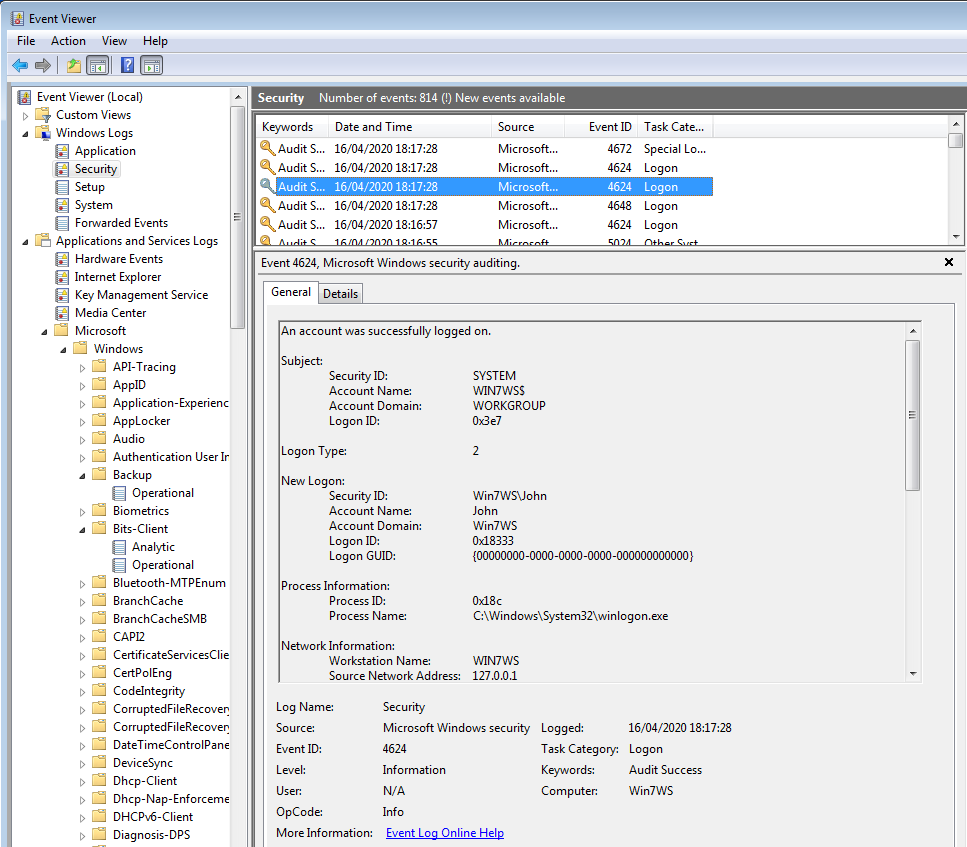
\includegraphics[scale=0.35]{images/evtx.png}
\end{frame}


\begin{frame}[fragile]
  \frametitle{2.3 Get support}
    \begin{itemize}
        \item Review logging policies
  \begin{lstlisting}[basicstyle=\tiny]
$ rip.pl -r SECURITY -p auditpol
.....
ystem:Other System Events                         S/F  
Logon/Logoff:Logon                                 S    
Logon/Logoff:Logoff                                S    
Logon/Logoff:Account Lockout                       S    
Logon/Logoff:IPsec Main Mode                       N    
Logon/Logoff:IPsec Quick Mode                      S    
Logon/Logoff:IPsec Extended Mode                   N    
Logon/Logoff:Special Logon                         N    
Logon/Logoff:Other Logon/Logoff Events             N    
Logon/Logoff:Network Policy Server                 S/F  
Object Access:File System                          N    
.....
  \end{lstlisting}
        \item Online:
            \begin{itemize}
                \item Microsoft TechNet
		\item \url{https://www.ultimatewindowssecurity.com/securitylog/encyclopedia/}
		\item \url{http://eventid.net/}
            \end{itemize}
    \end{itemize}
\end{frame}


\begin{frame}[fragile]
  \frametitle{2.4 Extracting and exploring event logs: Exercise}
  \begin{lstlisting}[basicstyle=\tiny]
Extracting event logs
---------------------
























_
  \end{lstlisting}
\end{frame}


\begin{frame}[fragile]
  \frametitle{2.4 Extracting and exploring event logs: Exercise}
  \begin{lstlisting}[basicstyle=\tiny]
Extracting event logs
---------------------

     mkdir evtx
     mkdir evtx/out

     mmls nps-2008-jean.raw
     sudo mount -o ro,offset=$((512*63)) nps-2008-jean.raw /media/sansforensics/casenps/

     cp /media/sansforensics/casenps/WINDOWS/system32/config/AppEvent.Evt evtx/
     cp /media/sansforensics/casenps/WINDOWS/system32/config/SecEvent.Evt evtx/
     cp /media/sansforensics/casenps/WINDOWS/system32/config/SysEvent.Evt evtx/
     ls -lh evtx/


Exploring event logs
--------------------









_
  \end{lstlisting}
\end{frame}


\begin{frame}[fragile]
  \frametitle{2.4 Extracting and exploring event logs: Exercise}
  \begin{lstlisting}[basicstyle=\tiny]
Extracting event logs
---------------------

     mkdir evtx
     mkdir evtx/out

     mmls image.raw
     sudo mount=o ro,offset=$((512*63)) image.raw/media/case1/

     cp /media/case1/WINDOWS/system32/config/AppEvent.Evt evtx/
     cp /media/case1/WINDOWS/system32/config/SecEvent.Evt evtx/
     cp /media/case1/WINDOWS/system32/config/SysEvent.Evt evtx/
     ls -lh evtx/


Exploring event logs
--------------------

     sudo apt install libevt-utils

     evtinfo evtx/AppEvent.Evt
     evtinfo evtx/SecEvent.Evt
     evtinfo evtx/SysEvent.Evt

     evtexport AppEvent.Evt | less
     evtexport SysEvent.Evt | less
  \end{lstlisting}
\end{frame}


\begin{frame}[fragile]
  \frametitle{2.4 Extracting and exploring event logs}
	\url{https://eventlogxp.com/}
    \includegraphics[scale=0.27]{images/evtx2.png}
\end{frame}


\begin{frame}[fragile]
	\frametitle{2.5 Example \texttt{.evtx}}
    \begin{itemize}
        \item Logon Success
  \begin{lstlisting}[basicstyle=\tiny]
$ evtxexport Security.evtx | less
.....
Event number          : 668
Written time          : Apr 15, 2019 12:58:33.650031000 UTC
Event level           : Information (0)
Computer name         : Win7WS
Source name           : Microsoft-Windows-Security-Auditing
Event identifier      : 0x00001210 (4624)
Number of strings     : 20
String: 1             : S-1-5-18
String: 2             : WIN7WS$
String: 3             : WORKGROUP
String: 4             : 0x00000000000003e7
String: 5             : S-1-5-21-3408732720-2018246097-660081352-1000
String: 6             : John
String: 7             : Win7WS
String: 9             : 2
.....
String: 17            : 0x0000018c
String: 18            : C:\Windows\System32\winlogon.exe
String: 19            : 127.0.0.1
  \end{lstlisting}
        \item Logon Fail
  \begin{lstlisting}[basicstyle=\tiny]
$ evtxexport Security.evtx | grep 4625
  \end{lstlisting}
    \end{itemize}
\end{frame}


\begin{frame}[fragile]
	\frametitle{2.5 Example \texttt{.evtx}}
    \includegraphics[scale=0.4]{images/f14_logonType.png}
\end{frame}


\begin{frame}[fragile]
  \frametitle{2.6 Other log files}
    \begin{itemize}
	\item \texttt{/Windows/setuplog.txt}
        \begin{itemize}
            \item Untill WinXP, when Windows is installed
        \end{itemize}
	\item \texttt{/Windows//Debug/netsetup.log}
        \begin{itemize}
            \item Untill WinXP, when Windows is installed
        \end{itemize}
	\item \texttt{/Windows/setupact.log}
        \begin{itemize}
            \item Graphical part of setup process
  \begin{lstlisting}[basicstyle=\tiny]
2019-04-05 11:39:56, Info  CBS Starting the TrustedInstaller main loop.
2019-04-05 11:39:56, Info  CBS TrustedInstaller service starts successfully.
2019-04-05 11:39:56, Info  CBS Setup in progress, aborting startup processing checks.
2019-04-05 11:39:56, Info  CBS Startup processing thread terminated normally
    \end{lstlisting}
	\end{itemize}
	\item \texttt{/Windows/setupapi.log}
  \begin{lstlisting}[basicstyle=\tiny]
/Windows/inf/setupapi.dev.log
/Windows/inf/setupapi.app.log
/Windows/inf/setupapi.offline.log
    \end{lstlisting}
	\item \texttt{/Windows/Tasks/SCHEDLGU.TXT}
        \begin{itemize}
            \item Task Scheduler Log
	\end{itemize}
    \end{itemize}
\end{frame}


\begin{frame}[fragile]
	\frametitle{2.7 Exercise: Automated tools}
  \begin{lstlisting}[basicstyle=\tiny]

     Example: Chainsaw
     =================
     
     wget https://github.com/WithSecureLabs/chainsaw/releases/
                  download/v2.10.1/chainsaw_all_platforms+rules.zip

     7z x chainsaw_all_platforms+rules.zip
     cd chainsaw
     chmod +x ./chainsaw_x86_64-unknown-linux-gnu
     git clone https://github.com/sbousseaden/EVTX-ATTACK-SAMPLES.git 

     ./chainsaw_x86_64-unknown-linux-gnu hunt EVTX-ATTACK-SAMPLES/ -s sigma/
          --mapping mappings/sigma-event-logs-all.yml | less


     [+] Loading detection rules from: sigma/
     [!] Loaded 3336 detection rules (490 not loaded)
     [+] Loading forensic artefacts from: EVTX-ATTACK-SAMPLES/Command 
         and Control, 2 (extensions: .evt, .evtx)



     Challenge: Hayabusa
     ===================

     https://github.com/Yamato-Security/hayabusa
  \end{lstlisting}
\end{frame}





%
% This work is licensed under a Creative Commons Attribution-ShareAlike 4.0 International License.
% http://creativecommons.org/licenses/by-sa/4.0/
%

% DO NOT COMPILE THIS FILE DIRECTLY!
% This is included by the other .tex files.


\begin{frame}
    \includegraphics[scale=.3]{images/logo-circl-Forensics.png}
    \begin{itemize}
        \item[]
        \item[]
        \item[] 3. Other Windows Artifacts
    \end{itemize}
\end{frame}


\begin{frame}[fragile]
  \frametitle{3.1 Recycle Bin - User support to undelete}
    \begin{itemize}
        \item Files move to Recycle Bin:
            \begin{itemize}
                \item Moved by mouse
		\item Right click: \texttt{Delete}
            \end{itemize}
        \item Not move to Recycle Bin:
            \begin{itemize}
		    \item Right click: \texttt{Delete + SHIFT}
		    \item Command line: \texttt{del}
		\item Files on network shares
            \end{itemize}
        \item NukeOnDelete
            \begin{itemize}
		    \item \texttt{HKEY\_USERS/\_UUID\_/Software/Microsoft/Windows/CurrentVers}
		    \item[]\texttt{ion/Explorer/BitBucket/Volume/\{\_Volume ID\_\}/NukeOnDelete}
                    \includegraphics[scale=.3]{images/nukeOD.png}
            \end{itemize}
    \end{itemize}
\end{frame}


\begin{frame}[fragile]
  \frametitle{3.1 Recycle Bin - Life-Investigate}
    \begin{itemize}
        \item Play script: \texttt{TextFile.txt} 
            \begin{itemize}
		\item 2019-04-30 17:31:57 UTC+2:  Born
		\item 2019-04-30 17:34:44 UTC+2:  Content Modified
		\item 2019-04-30 17:35:32 UTC+2:  Deleted
		\item[]
            \end{itemize}
        \item Analyze Recycle.Bin:
        \item[] \includegraphics[scale=.45]{images/f15_recycle.png}
    \end{itemize}
\end{frame}


\begin{frame}[fragile]
  \frametitle{3.1 Recycle Bin - Forensics}
    \begin{itemize}
        \item Play script: \texttt{TextFile.txt} 
            \begin{itemize}
		\item 2019-04-30 17:31:57 UTC+2:  Born
		\item 2019-04-30 17:34:44 UTC+2:  Content Modified
		\item 2019-04-30 17:35:32 UTC+2:  Deleted
		\item[]
            \end{itemize}
        \item Analyze \texttt{Recycle.Bin} directory:
  \begin{lstlisting}[basicstyle=\tiny]
/$Recycle.Bin/S-1-5-21-3408732720-2018246097-660081352-1000/
	129 Apr  5 11:46  desktop.ini
	544 Apr 30 17:35 '$IOMHI9A.txt'
	320 Apr 30 17:34 '$ROMHI9A.txt'


strings -el \$IOMHI9A.txt 
	C:\Users\John\Documents\recycleTest\TestFile.txt


strings \$ROMHI9A.txt 
		Test File
		=========
	This is a test file. It is just created to test Forensic
	Artifacts for the 'Recycle Bin'.
	.....
  \end{lstlisting}
    \end{itemize}
\end{frame}


\begin{frame}[fragile]
  \frametitle{3.1 Recycle Bin - Forensics}
    \begin{itemize}
        \item Play script: \texttt{TextFile.txt} 
            \begin{itemize}
		\item 2019-04-30 17:31:57 UTC+2:  Born
		\item 2019-04-30 17:34:44 UTC+2:  Content Modified
		\item 2019-04-30 17:35:32 UTC+2:  Deleted
		\item[]
            \end{itemize}
        \item File system timeline \texttt{Recycle.Bin} directory:
  \begin{lstlisting}[basicstyle=\tiny]
Tue Apr 30 2019 17:31:57
     320 ...b   47164-128-1 /$Recycle.Bin/S-1-5-21- ..... -1000/$ROMHI9A.txt


Tue Apr 30 2019 17:34:44
     320 ma..   47164-128-1 /$Recycle.Bin/S-1-5-21- ..... -1000/$ROMHI9A.txt


Tue Apr 30 2019 17:35:32
     544 macb   44155-128-1 /$Recycle.Bin/S-1-5-21- ..... -1000/$IOMHI9A.txt
      48 mac.   47022-144-1 /Users/John/Documents/recycleTest
     320 ..c.   47164-128-1 /$Recycle.Bin/S-1-5-21- ..... -1000/$ROMHI9A.txt
     376 mac.    9632-144-1 /$Recycle.Bin/S-1-5-21- ..... -1000
  \end{lstlisting}
    \end{itemize}
\end{frame}


\begin{frame}[fragile]
	\frametitle{3.1 Recycle Bin - Filename \& Extension}
    \includegraphics[scale=.31]{images/recycleEx.png}
\end{frame}


\begin{frame}[fragile]
  \frametitle{3.2 LNK Files}
    \begin{itemize}
        \item Link or shortcut to files, applications, resources
        \item User activity: Files access
        \begin{itemize}
            \item Local
            \item Network shares
            \item Appached devices
        \end{itemize}
        \item LNK file remain after target file is deleted
        \item[]
    \end{itemize}
  \begin{lstlisting}[basicstyle=\tiny]
Thu May 02 2019 14:54:02
     280 ...b       43701-144-1 /Users/John/Documents/LNK
 

Thu May 02 2019 14:54:28
      66 macb       43702-128-1 /Users/John/Documents/LNK/Test.txt


    1573 macb       43922-128-4 /Users/John/AppData/Roaming/Microsoft/
    				    Windows/Recent/LNK.lnk


    2779 macb       43716-128-4 /Users/John/AppData/Roaming/Microsoft/
    				    Windows/Recent/Test.txt.lnk
  \end{lstlisting}
\end{frame}


\begin{frame}[fragile]
  \frametitle{3.2 LNK Files}
    \begin{itemize}
        \item Information inside LNK files
        \begin{itemize}
            \item Target file MAC times
            \item Target file size
            \item Target file path
            \item Volume information
        \end{itemize}
        \item[]
    \end{itemize}
  \begin{lstlisting}[basicstyle=\tiny]
exiftool Test.txt.lnk
	...
	Create Date         : 2019:05:02 14:54:28+02:00
	Access Date         : 2019:05:02 14:54:28+02:00
	Modify Date         : 2019:05:02 14:54:28+02:00
	Target File Size    : 66
	Icon Index          : (none)
	Run Window          : Normal
	Hot Key             : (none)
	Drive Type          : Fixed Disk
	Volume Label        :
	Local Base Path     : C:\Users\
	Net Name            : 8
	Net Provider Type   : Unknown (0x20000)
	Relative Path       : ..\..\..\..\..\Documents\Test\Test.txt
	Working Directory   : C:\Users\John\Documents\Test
	Machine ID          : john-pc
  \end{lstlisting}
\end{frame}


\begin{frame}[fragile]
  \frametitle{3.2 LNK Files: Exercise}
    \begin{itemize}
	    \item[] Extract and investigate LNK file for document: 'm57biz.xls'
    \end{itemize}
  \begin{lstlisting}[basicstyle=\tiny]
Prepration work:
----------------







  















_ 
  \end{lstlisting}
\end{frame}


\begin{frame}[fragile]
  \frametitle{3.2 LNK Files: Exercise}
    \begin{itemize}
	    \item[] Extract and investigate LNK file for document: 'm57biz.xls'
    \end{itemize}
  \begin{lstlisting}[basicstyle=\tiny]
Prepration work:
----------------

  sudo mount -o ro,offset=$((512*63)) image.raw /media/case1
  mkdir lnk


 Copy LNK file:
 --------------
  















_ 
  \end{lstlisting}
\end{frame}


\begin{frame}[fragile]
  \frametitle{3.2 LNK Files: Exercise}
    \begin{itemize}
	    \item[] Extract and investigate LNK file for document: 'm57biz.xls'
    \end{itemize}
  \begin{lstlisting}[basicstyle=\tiny]
Prepration work:
----------------

  sudo mount -o ro,offset=$((512*63)) image.raw /media/case1
  mkdir lnk


 Copy LNK file:
 --------------
  
  cp /media/case1/Documents\ and\ Settings/Jean/Recent/m57biz.lnk lnk/


Investigate with exiftool:
--------------------------










_ 
  \end{lstlisting}
\end{frame}


\begin{frame}[fragile]
  \frametitle{3.2 LNK Files: Exercise}
    \begin{itemize}
	    \item[] Extract and investigate LNK file for document: 'm57biz.xls'
    \end{itemize}
  \begin{lstlisting}[basicstyle=\tiny]
Prepration work:
----------------

  sudo mount -o ro,offset=$((512*63)) image.raw /media/case1
  mkdir lnk


 Copy LNK file:
 --------------
  
  cp /media/case1/Documents\ and\ Settings/Jean/Recent/m57biz.lnk lnk/


Investigate with exiftool:
--------------------------

  exiftool lnk/m57biz.lnk
     .....
     File Attributes                 : Archive
     Create Date                     : 2008:07:20 01:28:03+00:00
     Access Date                     : 2008:07:20 01:28:03+00:00
     Modify Date                     : 2008:07:20 01:28:03+00:00
     Target File Size                : 291840
     Drive Type                      : Fixed Disk
     Local Base Path                 : C:\Documents and Settings\Jean\Desktop\m57biz.xls
_    Machine ID                      : jean-13fbf038a3
  \end{lstlisting}
\end{frame}


\begin{frame}[fragile]
  \frametitle{3.3 Jump Lists}
    \begin{itemize}
        \item Introduced with Windows 7
	\item Similar \texttt{Recent} folder
        \item Recently opened documents / application
	\item Makes them accessible at Windows main menu
	\item[]
        \includegraphics[scale=.3]{images/jl.png}
	\item[] \scriptsize{\texttt{AppData/Roaming/Microsoft/Windows/Recent/AutomaticDestinations}}
	\item[] \scriptsize{\texttt{AppData/Roaming/Microsoft/Windows/Recent/CustomDestinations}}
    \end{itemize}
\end{frame}


\begin{frame}[fragile]
  \frametitle{3.3 Jump Lists}
    \begin{itemize}
        \item File names start with 16 hex characters $\to$ JumpList ID
	\item File names end with \texttt{.xxxDestinations-ms}
	\item[]
  \begin{lstlisting}[basicstyle=\tiny]
C:> dir \Users\John\AppData\Roaming\Microsoft\Windows\Recent\AutomaticDestinations

04/05/2020  12:50            33 792 1b4dd67f29cb1962.automaticDestinations-ms
14/06/2019  16:43             4 608 28c8b86deab549a1.automaticDestinations-ms
10/04/2019  14:32            29 696 6824f4a902c78fbd.automaticDestinations-ms
10/04/2020  14:12             9 216 7e4dca80246863e3.automaticDestinations-ms
04/05/2020  12:50             8 704 918e0ecb43d17e23.automaticDestinations-ms
10/04/2019  14:30             3 072 b74736c2bd8cc8a5.automaticDestinations-ms
09/04/2019  14:43             6 144 de48a32edcbe79e4.automaticDestinations-ms
  \end{lstlisting}
	\item Each Hex value correspond to an fixed application
	\item \texttt{918e0ecb43d17e23 = Notepad.exe}
	\item[]
	\item[] \tiny{$\to$ \url{https://github.com/EricZimmerman/JumpList/blob/master/JumpList/Resources/AppIDs.txt}}
    \end{itemize}
\end{frame}


\begin{frame}[fragile]
  \frametitle{3.3 Jump Lists}
    \begin{itemize}
        \item Exercise: Identify applications
  \begin{lstlisting}[basicstyle=\tiny]
cd JumpLists/AutomaticDestinations/
ls -l

    1b4dd67f29cb1962.automaticDestinations-ms --> 
    28c8b86deab549a1.automaticDestinations-ms --> 
    6824f4a902c78fbd.automaticDestinations-ms --> 
    7e4dca80246863e3.automaticDestinations-ms --> 
    918e0ecb43d17e23.automaticDestinations-ms --> 
    b74736c2bd8cc8a5.automaticDestinations-ms --> 
    de48a32edcbe79e4.automaticDestinations-ms --> 
  \end{lstlisting}
	\item Exercise: Analyze the Notepad Jump List file
  \begin{lstlisting}[basicstyle=\tiny]











-
  \end{lstlisting}
    \end{itemize}
\end{frame}


\begin{frame}[fragile]
  \frametitle{3.3 Jump Lists}
    \begin{itemize}
        \item Exercise: Identify applications
  \begin{lstlisting}[basicstyle=\tiny]
cd JumpLists/AutomaticDestinations/
ll

    1b4dd67f29cb1962.automaticDestinations-ms --> Windows Explorer
    28c8b86deab549a1.automaticDestinations-ms --> Internet Explorer 8
    6824f4a902c78fbd.automaticDestinations-ms --> Firefox 64.x
    7e4dca80246863e3.automaticDestinations-ms --> Control Panel
    918e0ecb43d17e23.automaticDestinations-ms --> Notepad (32-bit)
    b74736c2bd8cc8a5.automaticDestinations-ms --> WinZip
    de48a32edcbe79e4.automaticDestinations-ms --> Acrobat Reader 15.x
  \end{lstlisting}
	\item Exercise: Analyze the Notepad Jump List file
  \begin{lstlisting}[basicstyle=\tiny]











-
  \end{lstlisting}
    \end{itemize}
\end{frame}


\begin{frame}[fragile]
  \frametitle{3.3 Jump Lists}
    \begin{itemize}
        \item Exercise: Identify applications
  \begin{lstlisting}[basicstyle=\tiny]
cd JumpLists/AutomaticDestinations/
ll

    1b4dd67f29cb1962.automaticDestinations-ms --> Windows Explorer
    28c8b86deab549a1.automaticDestinations-ms --> Internet Explorer 8
    6824f4a902c78fbd.automaticDestinations-ms --> Firefox 64.x
    7e4dca80246863e3.automaticDestinations-ms --> Control Panel
    918e0ecb43d17e23.automaticDestinations-ms --> Notepad (32-bit)
    b74736c2bd8cc8a5.automaticDestinations-ms --> WinZip
    de48a32edcbe79e4.automaticDestinations-ms --> Acrobat Reader 15.x
  \end{lstlisting}
	\item Exercise: Analyze the Notepad Jump List file
  \begin{lstlisting}[basicstyle=\tiny]
7z l 918e0ecb43d17e23.automaticDestinations-ms
        Date      Time    Attr         Size   Compressed  Name
     ------------------- ----- ------------ ------------  -------
                         .....         1398         1408  2
                         .....         1368         1408  1
                         .....          436          448  4
                         .....          392          448  3

--> file
--> exiftool
--> strings 
7z x 918e0ecb43d17e23.automaticDestinations-ms
strings -el DestList
  \end{lstlisting}
    \end{itemize}
\end{frame}


\begin{frame}[fragile]
  \frametitle{3.4 Prefetch Files}
    \begin{itemize}
	\item Application prefetching since XP
        \begin{itemize}
            \item Monitor an application when it starts
            \item Collect information about resources needed
            \item Wait 10sec after application started
	    \item[] $\to$ Know where to find the resources
            \item[] $\to$ Better performance: App launch faster
            \item[] $\to$ Better user experience
	    \item[]
        \end{itemize}
	\item Forensics value:
        \begin{itemize}
            \item Proof an application was started
            \begin{itemize}
                \item Secondary artifact
                \item Created by the OS
                \item Not deleted by the attacker
            \end{itemize}
            \item Even if the application don't exists anymore
            \item And more .....
        \end{itemize}
    \end{itemize}
\end{frame}


\begin{frame}[fragile]
  \frametitle{3.4 Prefetch Files}
    \begin{itemize}
        \item Example: From file system time line
  \begin{lstlisting}[basicstyle=\tiny]
Thu May 02 2019 14:52:40
    179712 .a..      10940-128-3 /Windows/notepad.exe

Thu May 02 2019 14:52:50
        56 mac.      42729-144-6 /Windows/Prefetch
     16280 macb      43700-128-4 /Windows/Prefetch/NOTEPAD.EXE-D8414F97.pf
  \end{lstlisting}
        \item Elements of the file name at \texttt{/Windows/Prefetch}
        \begin{itemize}
            \item Application name
            \item One way hash of path to the application
	    \item File extension: \texttt{.pf}
        \end{itemize}
        \item Information found inside a Prefetch file:
        \begin{itemize}
            \item Run count: How often application run
            \item Last time executed
            \item Application name incl. parameter
            \item Path to application and resources
        \end{itemize}
    \end{itemize}
\end{frame}


\begin{frame}[fragile]
  \frametitle{3.4 Prefetch Files}
    \begin{itemize}
        \item Parsing a Prefetch file
  \begin{lstlisting}[basicstyle=\tiny]
prefetch.py -f NOTEPAD.EXE-D8414F97.pf

	Executable Name: NOTEPAD.EXE
	Run count: 1
	Last Executed: 2019-05-02 12:52:40.339584

	Resources loaded:
	1:    \DEVICE\HARDDISKVOLUME2\WINDOWS\SYSTEM32\NTDLL.DLL
	2:    \DEVICE\HARDDISKVOLUME2\WINDOWS\SYSTEM32\KERNEL32.DLL
	3:    \DEVICE\HARDDISKVOLUME2\WINDOWS\SYSTEM32\APISETSCHEMA.DLL
	4:    \DEVICE\HARDDISKVOLUME2\WINDOWS\SYSTEM32\KERNELBASE.DLL
	.....
	.....
  \end{lstlisting}
        \item Additional benefits like:
        \begin{itemize}
            \item User folder where the malware got executed
            \item Compare Run count of different VSS could
	    \item[] $\to$ Behavior of user
        \end{itemize}
    \end{itemize}
\end{frame}


\begin{frame}[fragile]
  \frametitle{3.4 Prefetch Files: Exercise}
    \begin{itemize}
	    \item[] Extract and investigate the Excel prefetch file
	    \item[] 
    \end{itemize}
  \begin{lstlisting}[basicstyle=\tiny]
Copy prefetch file:
-------------------
  
    mkdir prefetch
    cp /media/sansforensics/casenps/WINDOWS/Prefetch/EXCEL.EXE-1C75F8D6.pf prefetch/


Investigate LNK file:
---------------------

    strings -el prefetch/EXCEL.EXE-1C75F8D6.pf | less


    pref.pl -f prefetch/EXCEL.EXE-1C75F8D6.pf

	File     : prefetch/EXCEL.EXE-1C75F8D6.pf
	Exe Path : \DEVICE\HARDDISKVOLUME1\PROGRAM FILES\MICROSOFT OFFICE\OFFICE\EXCEL.EXE
	Last Run : Sun Jul 20 01:27:40 2008
	Run Count: 2
  \end{lstlisting}
\end{frame}


\begin{frame}[fragile]
  \frametitle{3.5 XP Restore Points}
    \begin{itemize}
        \item Backup of:
        \begin{itemize}
	    \item Critical system files
	    \item Registry partially
            \item Local user profiles
            \item But NO user data!
        \end{itemize}
        \item Created automatically:
        \begin{itemize}
            \item Every 24 hours
            \item Windows Update
	    \item Installation of applications incl. driver
            \item Manually
        \end{itemize}
        \item For user: Useful to recover a broken system
        \item For analyst:
        \begin{itemize}
	    \item \texttt{rp.log}
            \item Description of the cause
            \item Time stamp
            \item State of the system at different times
        \end{itemize}
    \end{itemize}
\end{frame}


\begin{frame}[fragile]
  \frametitle{3.6 VSS - Volume Shadow Copy Service}
    \begin{itemize}
	    \item Backup Service
            \begin{itemize}
	         \item System files
	         \item User data files
	         \item Operates on block level
            \end{itemize}
	    \item On live system
            \begin{itemize}
	         \item Run CMD as administrator
  \begin{lstlisting}[basicstyle=\tiny]
>vssadmin list shadows /for=c:/
vssadmin 1.1 - Volume Shadow Copy Service administrative command-line tool
(C) Copyright 2001-2005 Microsoft Corp.

Contents of shadow copy set ID: {33eb3a7b-6d03-4045-aa70-37b714d49c72}
   Contained 1 shadow copies at creation time: 10/04/2019 16:06:30
      Shadow Copy ID: {34d9910b-ac1d-4b10-b282-89dde217d0fb}
         Original Volume: (C:)\\?\Volume{a62c8cd4-5786-11e9-a9fd-806e6f6e6963}\
         Shadow Copy Volume: \\?\GLOBALROOT\Device\HarddiskVolumeShadowCopy1
         Originating Machine: Win7WS
         Service Machine: Win7WS
         Provider: 'Microsoft Software Shadow Copy provider 1.0'
         Type: ClientAccessibleWriters
         Attributes: Persistent, Client-accessible, No auto release, Differential,
	 Auto recovered
  \end{lstlisting}
            \end{itemize}
  \end{itemize}
\end{frame}


\begin{frame}[fragile]
  \frametitle{3.6 VSS - Configuration}
	    \begin{itemize}
		    \item[] \scriptsize{\texttt{HKEY\_LOCAL\_MACHINE/SYSTEM/CurrentControlSet/services/VSS}}
		    \includegraphics[scale=.3]{images/VSSConfig2.png}
		    \item[]
	    \item[] \scriptsize{\texttt{HKEY\_LOCAL\_MACHINE/SYSTEM/CurrentControlSet/Control/BackupRestore}}
		    \includegraphics[scale=.3]{images/VSSConfig.png}
            \end{itemize}
\end{frame}


\begin{frame}[fragile]
  \frametitle{3.5 VSS - Analysis}
    \begin{itemize}
	    \item[] Analyze disk image
  \begin{lstlisting}[basicstyle=\tiny]
vshadowinfo -o $((512*206848)) 8d34ce.raw 

    Volume Shadow Snapshot information:
	Number of stores:	1

    Store: 1
	Identifier		: 237c8de3-5b99-11e9-9925-080027062798
	Shadow copy set ID	: 33eb3a7b-6d03-4045-aa70-37b714d49c72
	Creation time		: Apr 10, 2019 14:06:30.365699200 UTC
	Shadow copy ID		: 34d9910b-ac1d-4b10-b282-89dde217d0fb
	Volume size		: 11 GiB (12777947136 bytes)
	Attribute flags		: 0x0042000d
  \end{lstlisting}
	    \item[] Mounting VSC: A 2 step approach
  \begin{lstlisting}[basicstyle=\tiny]
sudo vshadowmount -o $((512*206848)) 8d34ce.raw /mount/vss/

sudo ls -l /mount/vss/
	-r--r--r-- 1 root root 12777947136 Jan  1  1970 vss1

sudo file /mount/vss/vss1
	/mount/vss/vss1: DOS/MBR boot sector, code offset 0x52+2, OEM-ID "NTFS 

sudo mount -o ro /mount/vss/vss1 /mnt/
  \end{lstlisting}
  \end{itemize}
\end{frame}



%
% This work is licensed under a Creative Commons Attribution-ShareAlike 4.0 International License.
% http://creativecommons.org/licenses/by-sa/4.0/
%

% DO NOT COMPILE THIS FILE DIRECTLY!
% This is included by the other .tex files.


\begin{frame}
    \includegraphics[scale=0.3]{images/logo-circl-Forensics.png}
    \begin{itemize}
        \item[]
        \item[]
        \item[] 4. Basic Malware Analysis
    \end{itemize}
\end{frame}


\begin{frame}[fragile]
  \frametitle{4.1 Introduction}
    \begin{itemize}
	    \item[] Take care: Self-Infection:
    	    \begin{itemize}
	    	\item Keep away from production
		\item Isolated machines (VMs)
		\item Network considerations
		\item[]
    	    \end{itemize}
	    \item[] Exchange of malware via email:
    	    \begin{itemize}
	    	\item Password protected archive
		\item Password: \texttt{infected}
		\item[]
    	    \end{itemize}
	    \item[] 5 Phases of analysis
            \begin{enumerate}
            	\item OSINT - Open Source Intelligence
		\item Automatic Analysis (Sandbox)
            	\item Static Analysis
		\item Dynamic Analysis (Behavioral Analysis)
            	\item Reverse Engineering
		\item[]
            \end{enumerate}
    \end{itemize}
\end{frame}


\begin{frame}[fragile]
  \frametitle{4.2 OSINT - IoCs}
    \begin{itemize}
	    \item Is the file \texttt{Form.exe} malicious?
            \item What it is doing?
    \end{itemize}
  \begin{lstlisting}[basicstyle=\tiny]
    ls -l Form.exe				                    189952 Form.exe
   md5sum Form.exe		                   a8371cb187d99711691ccbecf8f35657
  sha1sum Form.exe                         8dec32121d2f9f876c2b157451968796608d3dd5
sha256sum Form.exe 784560f38065089f1c61869f7ebdc58b0115d500e5113e6c09d1b4d885ccb340
  \end{lstlisting}
  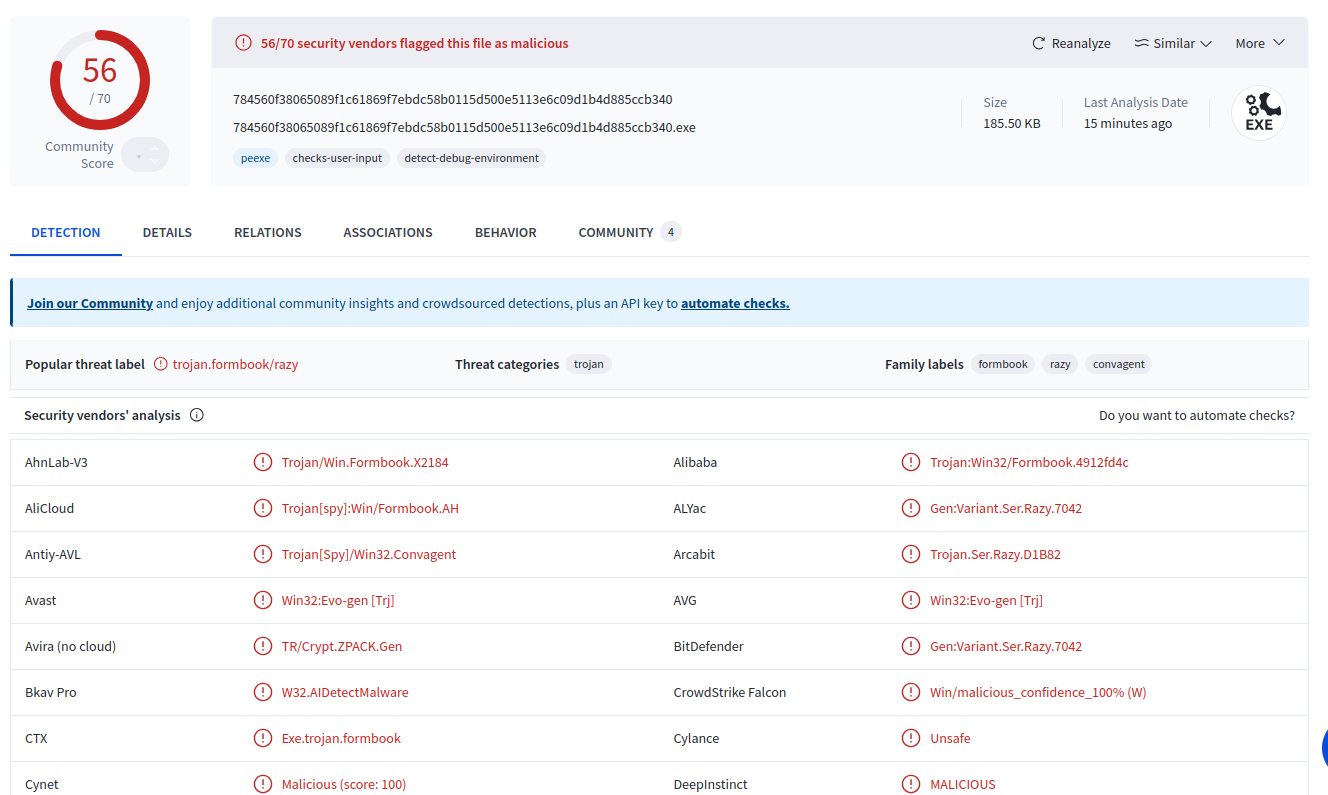
\includegraphics[scale=0.17]{images/VT_1.png}
\end{frame}


\begin{frame}[fragile]
  \frametitle{4.2 OSINT - Malpedia}
  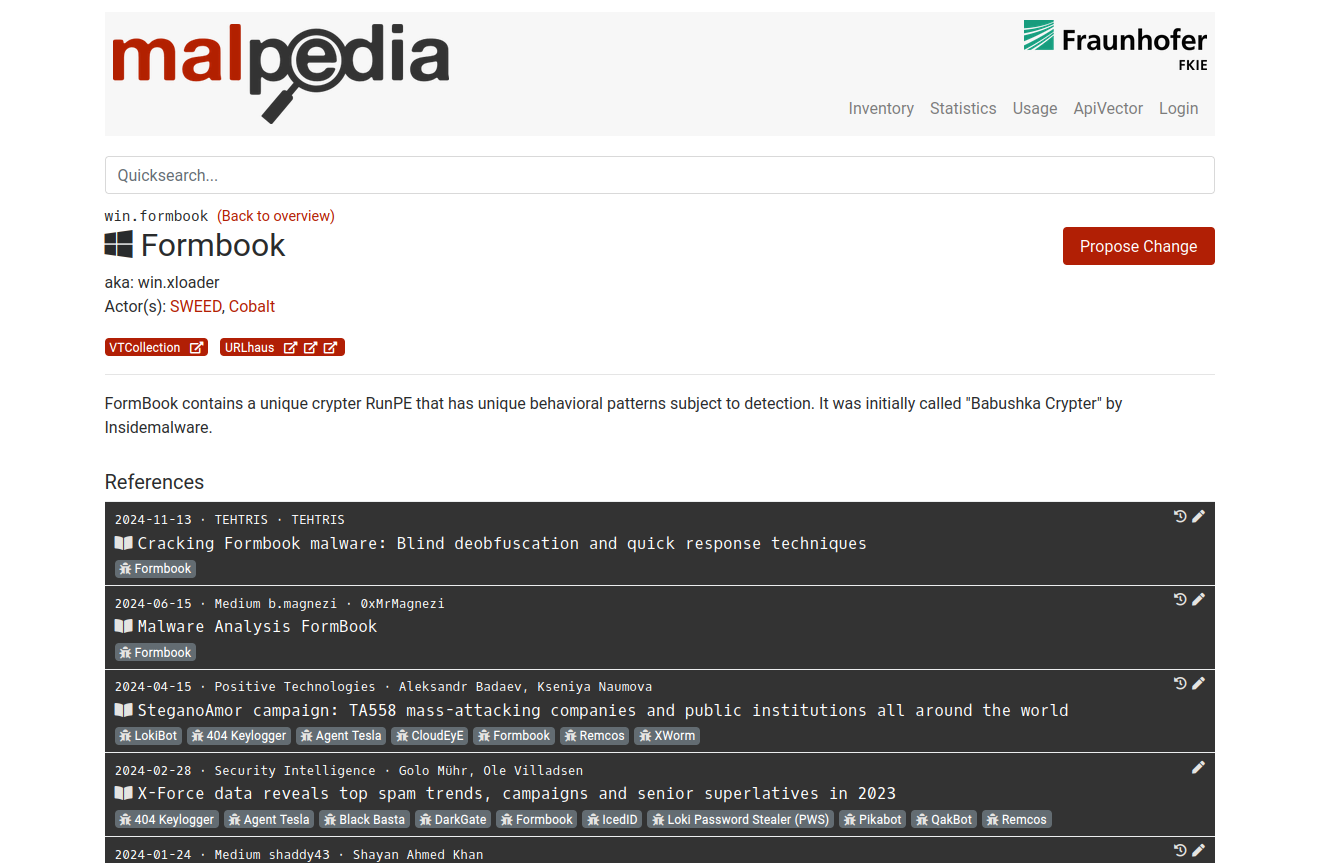
\includegraphics[scale=0.24]{images/malpedia.png}
\end{frame}


\begin{frame}[fragile]
  \frametitle{4.2 OSINT - VirusTotal Details}
  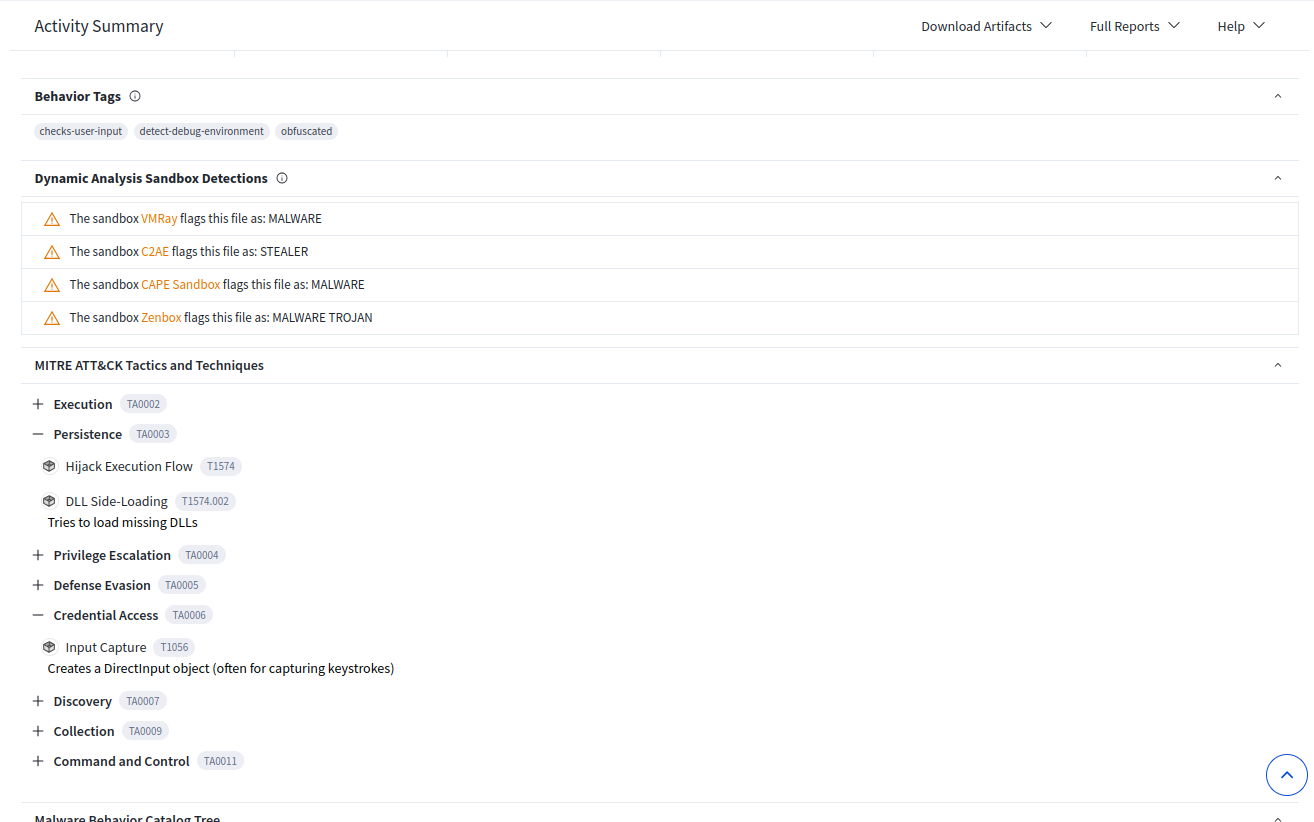
\includegraphics[scale=0.24]{images/VT_2.png}
\end{frame}


\begin{frame}[fragile]
  \frametitle{4.2 OSINT - abuse.ch - MalwareBazaar}
  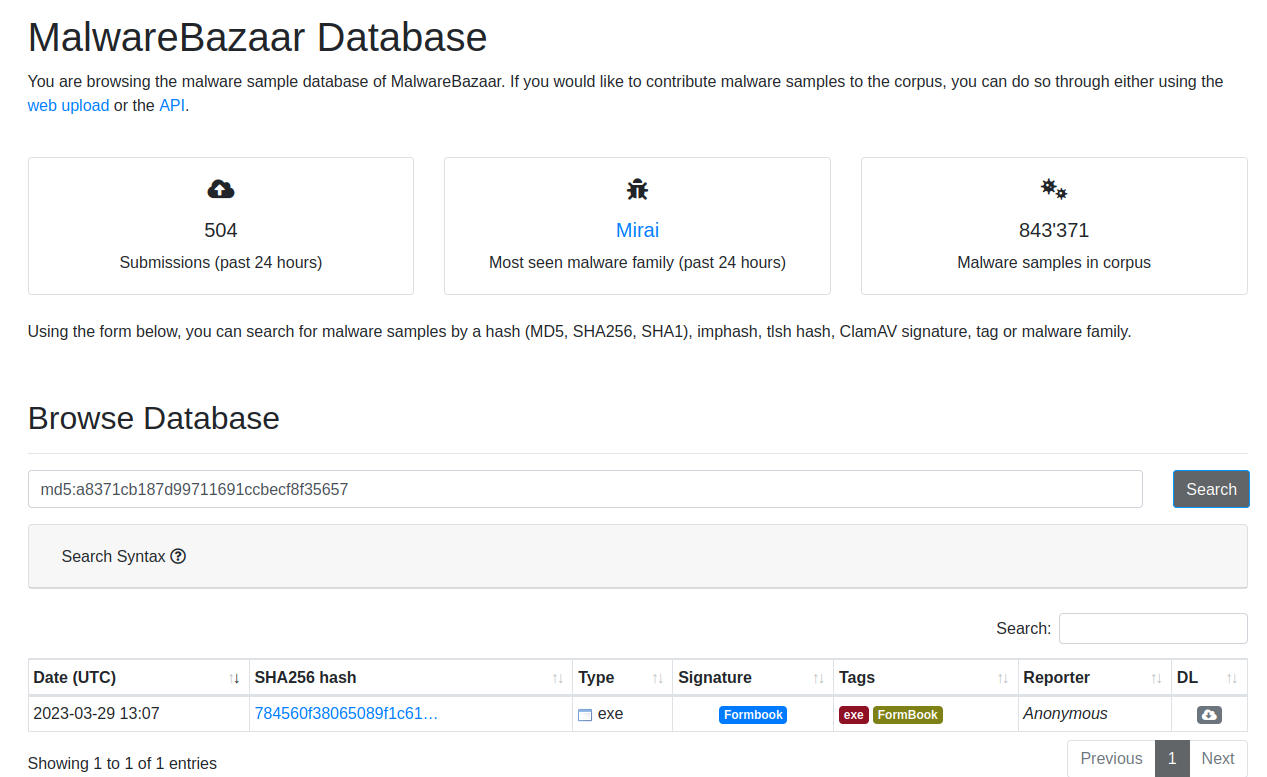
\includegraphics[scale=0.24]{images/mwBazaar.png}
\end{frame}


\begin{frame}[fragile]
  \frametitle{4.2 OSINT - MISPPriv}
  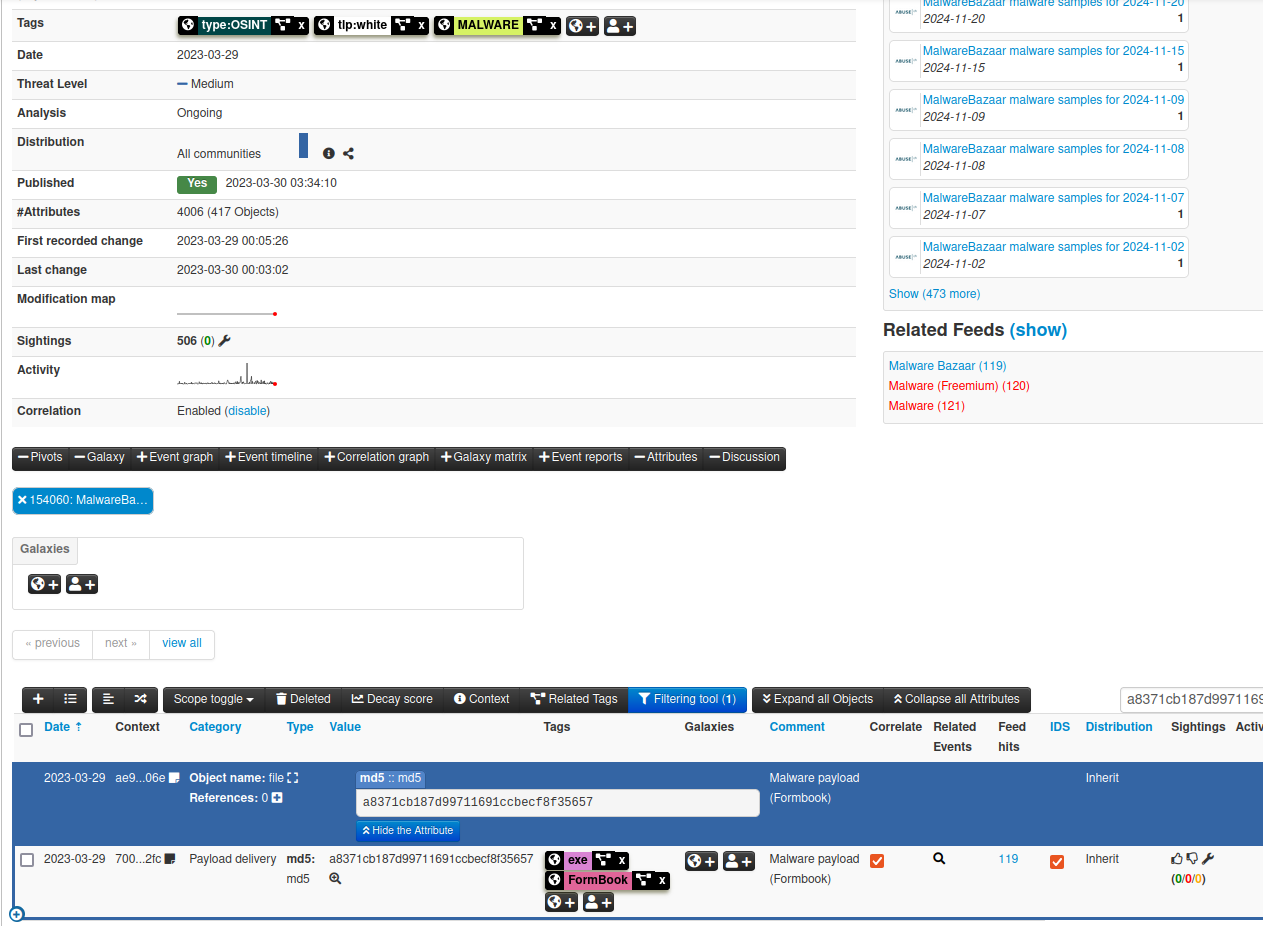
\includegraphics[scale=0.22]{images/misp.png}
\end{frame}


\begin{frame}[fragile]
  \frametitle{4.3 Sandbox - Joe}
  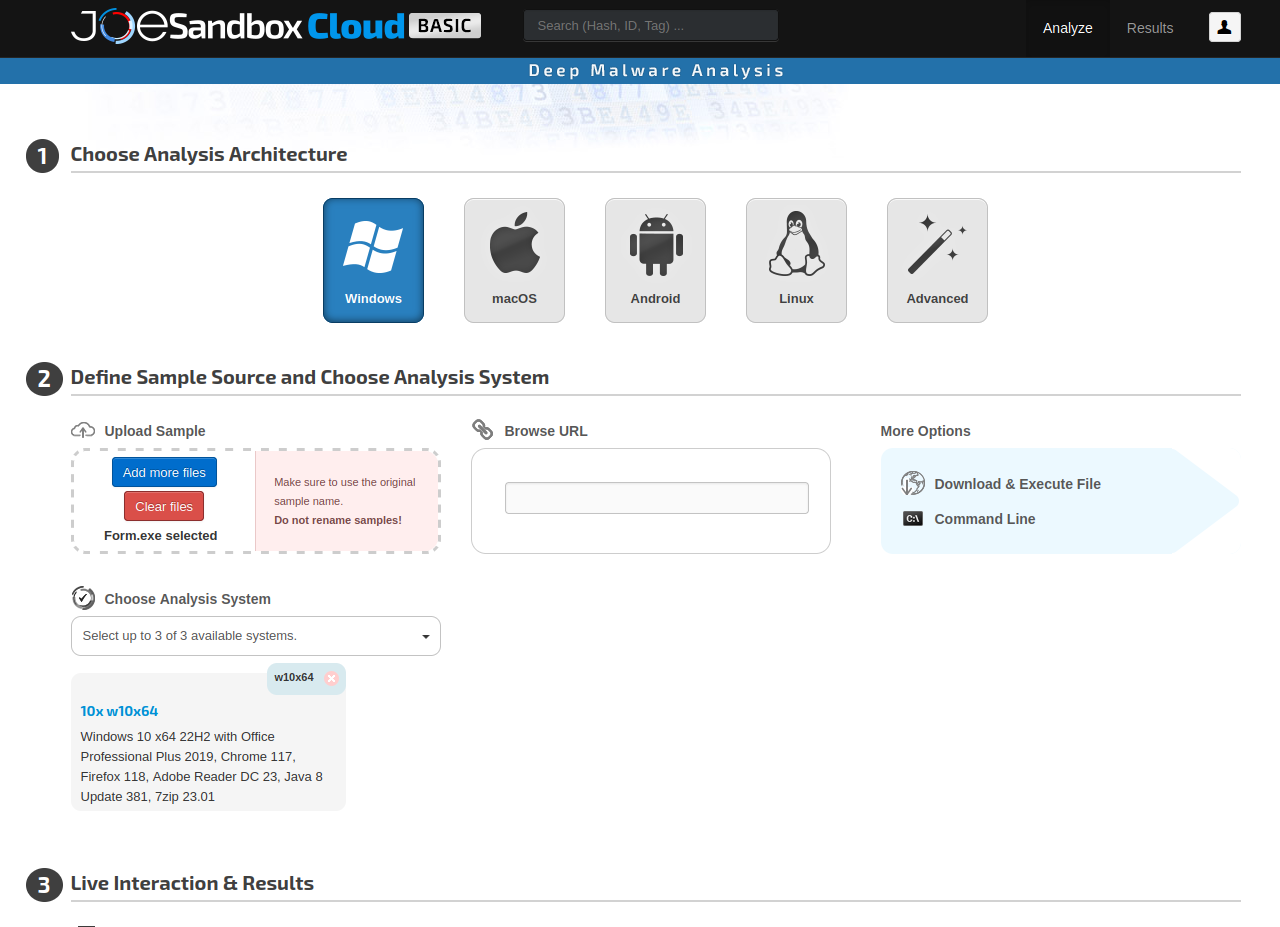
\includegraphics[scale=0.22]{images/joe1.png}
\end{frame}


\begin{frame}[fragile]
  \frametitle{4.3 Sandbox - Joe}
  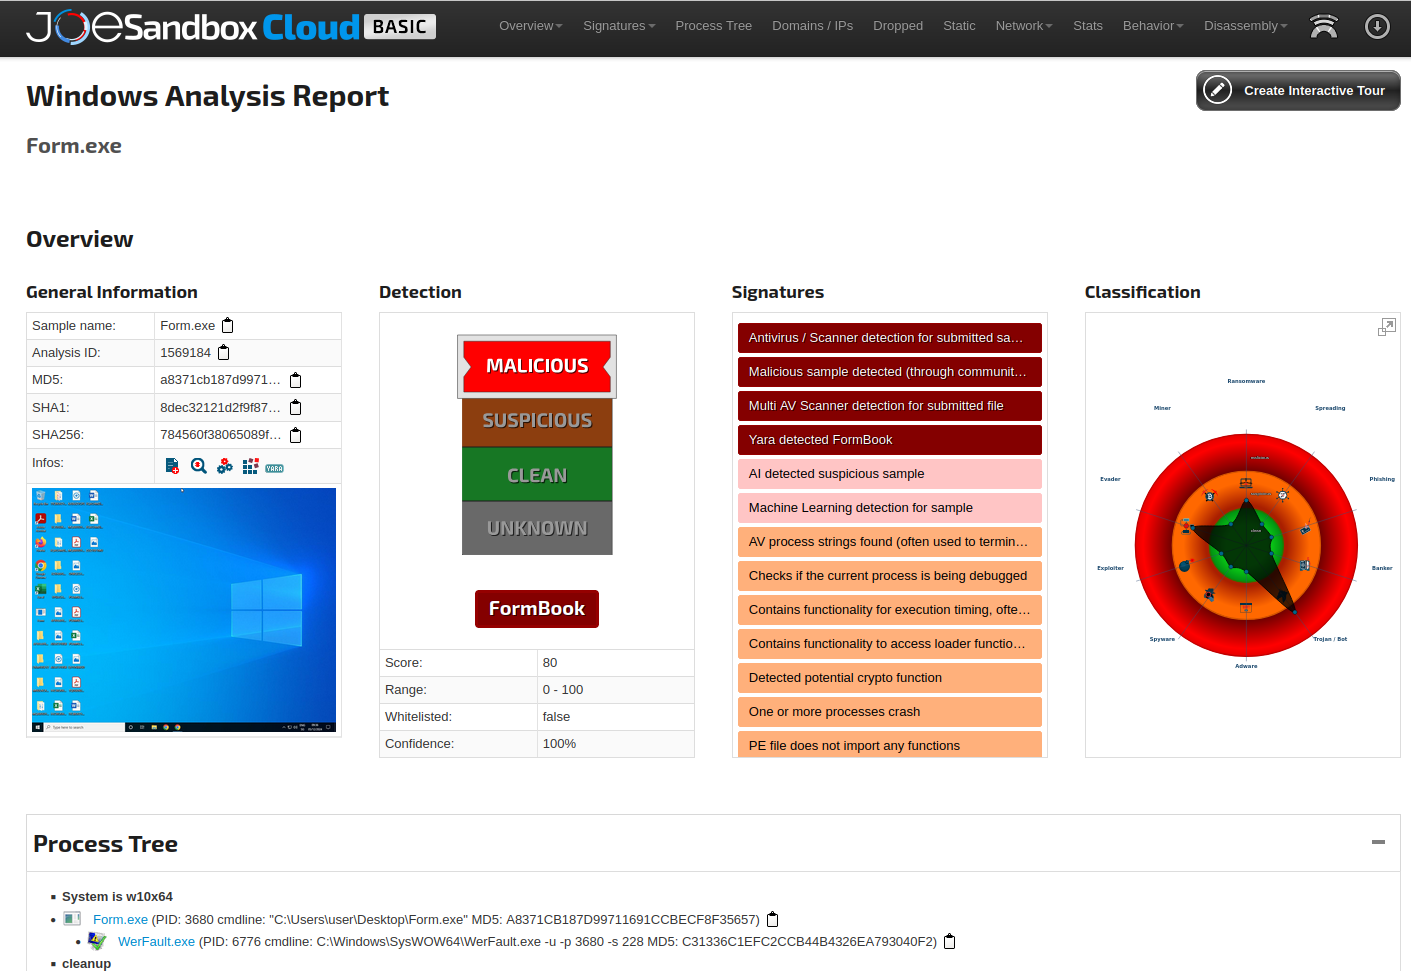
\includegraphics[scale=0.21]{images/joe2.png}
\end{frame}


\begin{frame}[fragile]
  \frametitle{4.3 Sandbox - Joe}
  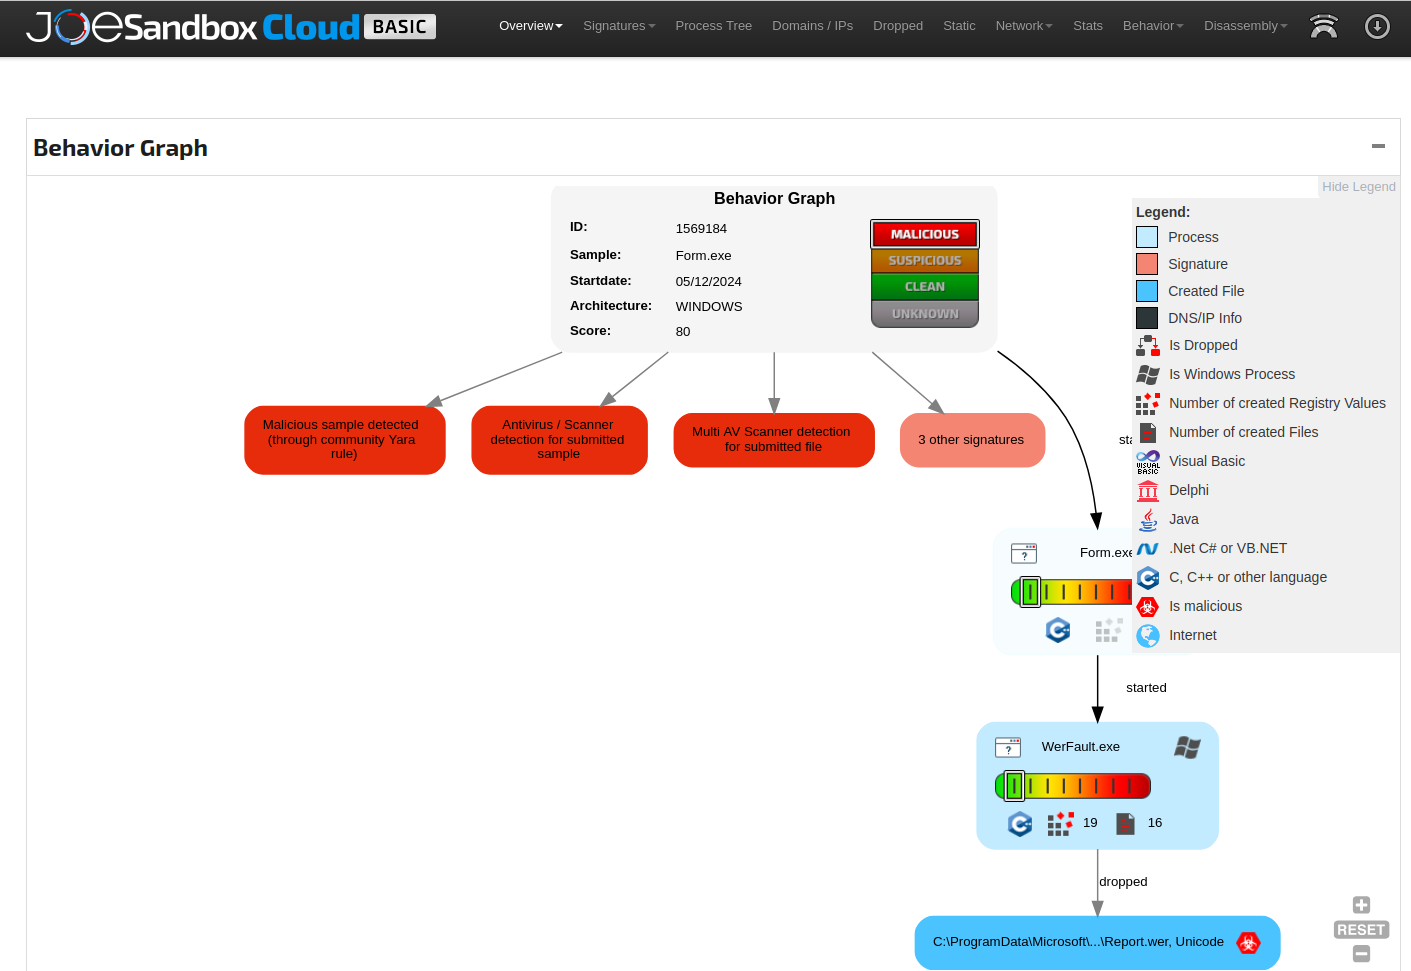
\includegraphics[scale=0.21]{images/joe3.png}
\end{frame}


\begin{frame}[fragile]
  \frametitle{4.3 Sandbox - Cuckoo3}
  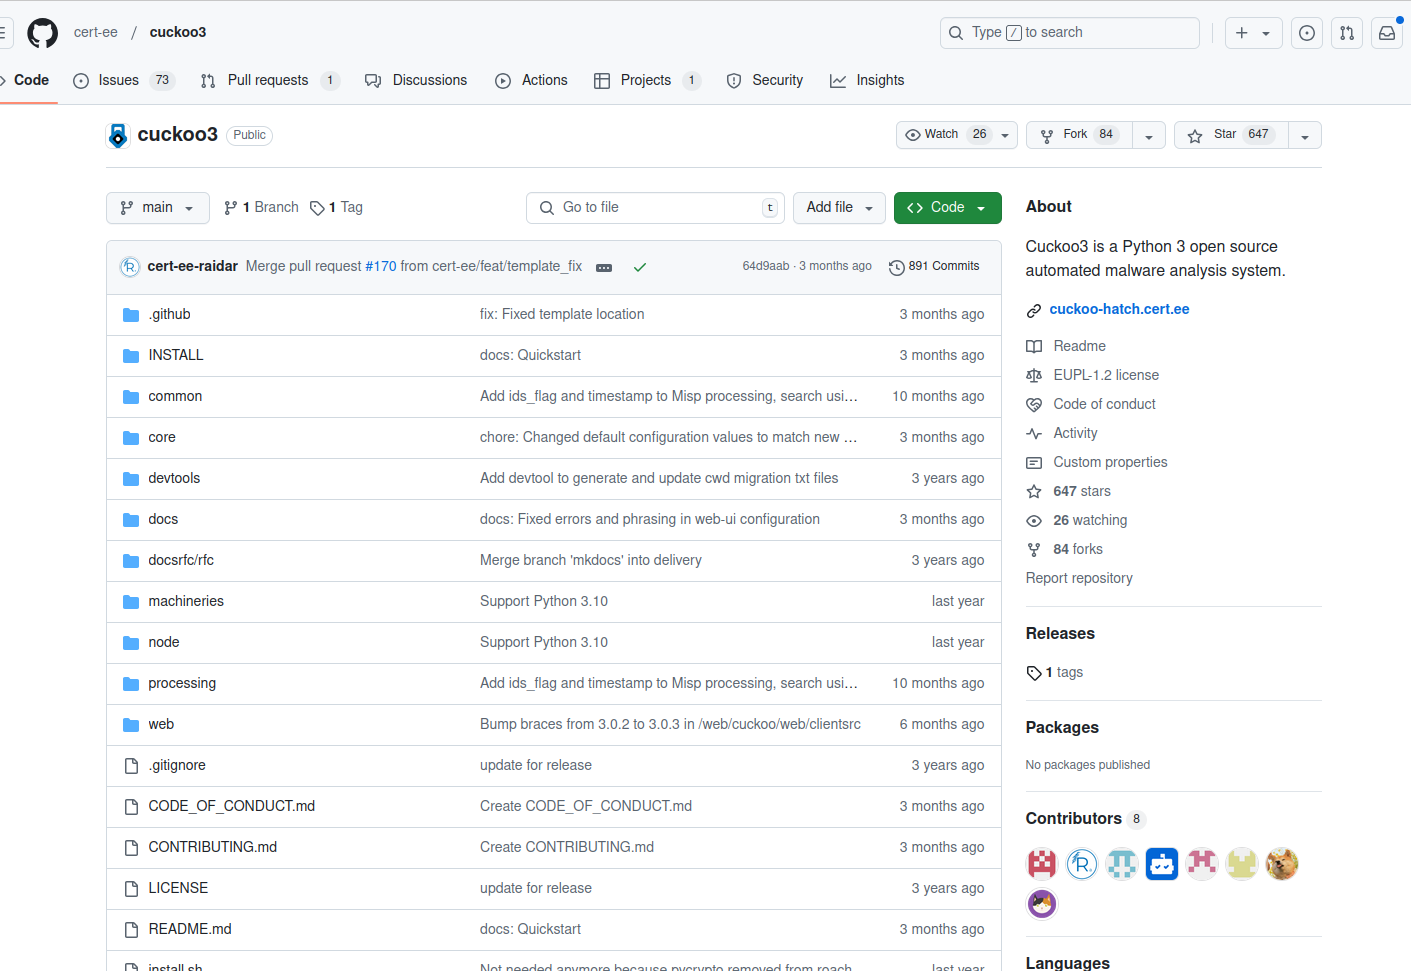
\includegraphics[scale=0.21]{images/cuckoo.png}
\end{frame}


\begin{frame}[fragile]
  \frametitle{4.4 Static Analysis}
    \begin{itemize}
        \item Malware delivery: Email
        \begin{itemize}
            \item Office documents
            \item PDF
            \item .EXE
        \end{itemize}
        \item Analyze:
        \begin{itemize}
            \item Hash values
            \item Strings
            \item Resources
            \item Imported functions
            \item Exported functions
            \item Certificate
            \item .....
        \end{itemize}
        \item[] $\to$ Capabilities of the malware
    \end{itemize}
\end{frame}


\begin{frame}[fragile]
  \frametitle{4.4 Static Analysis - Strings}
  \begin{lstlisting}[basicstyle=\tiny]
      pestr -n 7 Form.exe | less
      --------------------------
      !This program cannot be run in DOS mode.
      <Ar5<zw1<Zv
      EThis program cannot be run in DOS mode.
      :Yf/yZjP
      [)sk/Jo
      X|e^BZ8
      Rh%';,V


      pescan Form.exe
      ---------------
      file entropy:                    7.322160 (probably packed)
      fpu anti-disassembly:            no
      imagebase:                       normal
      entrypoint:                      normal
      DOS stub:                        normal
      TLS directory:                   not found
      timestamp:                       normal
      section count:                   1 (low)


      pesec Form.exe
      --------------
      ASLR:                            yes
      DEP/NX:                          yes
      SEH:                             yes
      Stack cookies (EXPERIMENTAL):    yes
  \end{lstlisting}
\end{frame}


\begin{frame}[fragile]
  \frametitle{4.4 Static Analysis - PE - Portable Execution format}
    \begin{itemize}
        \item Describe program files
        \item Contain:
        \begin{itemize}
            \item Meta data
            \item Instructions
            \item Text data
            \item Resources: Pictures and alike
        \end{itemize}
        \item Tell Windows how to load a program
        \item Provide resources to running program
        \item Provide resources like code signature
    \end{itemize}
  \begin{lstlisting}[basicstyle=\tiny]
      ---------------------------------------------
      |  1. DOS Header                            |
      |  2. PE Header                             |
      |  3. OPtional Header                       |
      |  4. Section Headers                       |
      |  5. .text Section (Program Code)          |
      |  6. .idata Section (Importd Libs)         |
      |  7. .rsrc Section (Strings, Images, ...)  |
      |  8. .reloc Section (Memory Translation)   |
      ---------------------------------------------
  \end{lstlisting}
\end{frame}


\begin{frame}[fragile]
  \frametitle{4.4 Static Analysis - PE - Basic Analysis}
  \begin{lstlisting}[basicstyle=\tiny]
file Form.exe
-------------
     Form.exe: PE32 executable (GUI) Intel 80386, for MS Windows


exiftool Form.exe
-----------------
     File Name                       : Form.exe
     File Size                       : 186 KiB
     .....
     File Type                       : Win32 EXE
     File Type Extension             : exe
     MIME Type                       : application/octet-stream
     Machine Type                    : Intel 386 or later, and compatibles
     Time Stamp                      : 2000:07:31 02:00:25+02:00
     Image File Characteristics      : Executable, 32-bit
     PE Type                         : PE32
     Linker Version                  : 11.0
     Code Size                       : 185856
     Initialized Data Size           : 0
     Uninitialized Data Size         : 0
     Entry Point                     : 0x12e0
     OS Version                      : 6.0
     Image Version                   : 0.0
     Subsystem Version               : 6.0
     Subsystem                       : Windows GUI
     Warning                         : Error processing PE data dictionary
  \end{lstlisting}
\end{frame}


\begin{frame}[fragile]
  \frametitle{4.4 Static Analysis - PE - Basic Analysis}
  \begin{lstlisting}[basicstyle=\tiny]
file Quotation.exe
------------------
     Quotation.exe: PE32 executable (GUI) Intel 80386, for MS Windows


exiftool Quotation.exe
----------------------  
     ...
     Machine Type                    : Intel 386 or later, and compatibles
     Time Stamp                      : 2005:08:14 14:47:46+02:00
     PE Type                         : PE32
     Linker Version                  : 6.0
     Code Size                       : 647168
     Initialized Data Size           : 32768
     Uninitialized Data Size         : 0
     Entry Point                     : 0x15f4
     OS Version                      : 4.0
     Character Set                   : Unicode
     Comments                        : Natcher
     Company Name                    : Glucosazone
     Legal Copyright                 : CRUSTER3
     Legal Trademarks                : Forearming
     Product Name                    : UNKLE
     File Version                    : 1.02.0009
     Product Version                 : 1.02.0009
     Internal Name                   : Aurous
     Original File Name              : Aurous.exe
  \end{lstlisting}
\end{frame}


\begin{frame}[fragile]
  \frametitle{4.4 Static Analysis - PE - Header}
  \begin{lstlisting}[basicstyle=\tiny]
readpe -H Form.exe
------------------

     DOS Header
         Magic number:                    0x5a4d (MZ)
         Bytes in last page:              144
         Pages in file:                   3
         .....

     Optional/Image header
         Magic number:                    0x10b (PE32)
         Linker major version:            11
         Linker minor version:            0
         Size of .text section:           0x2d600
         Size of .data section:           0
         Size of .bss section:            0
         Entrypoint:                      0x12e0
         Address of .text section:        0x1000
         Address of .data section:        0x2f000
         ImageBase:                       0x400000
         Alignment of sections:           0x1000
         Alignment factor:                0x200
         .....
	 Size of image:                   0x2f000
         Size of headers:                 0x200
         Checksum:                        0
         Subsystem required:              0x2 (IMAGE_SUBSYSTEM_WINDOWS_GUI)
         DLL characteristics:             0x8140
         .....
  \end{lstlisting}
\end{frame}


\begin{frame}[fragile]
  \frametitle{4.4 Static Analysis - PE - Imported Functions}
  \begin{lstlisting}[basicstyle=\tiny]
readpe -i ../1.exe
------------------
    Library
        Name:                            COMCTL32.dll
        Functions
                Name:                            ImageList_GetDragImage
                Name:                            ImageList_Merge
                Name:                            ImageList_SetOverlayImage
                Name:                            UninitializeFlatSB
                Name:                            ImageList_DragEnter
    Library
        Name:                            OLEAUT32.dll
        Functions
            Function
                Ordinal:                         294
    Library
        Name:                            ADVAPI32.dll
        Functions
                Name:                            RegOpenKeyExA
                Name:                            MapGenericMask
                Name:                            AdjustTokenGroups
                Name:                            SetSecurityDescriptorDacl
                Name:                            GetSecurityDescriptorLength
                Name:                            StartServiceA
                Name:                            OpenServiceA
    Library
        Name:                            MSVCRT.dll
        Functions
                Name:                            _mbsspnp
         .....
  \end{lstlisting}
\end{frame}


\begin{frame}[fragile]
  \frametitle{4.4 Static Analysis - PE - Resources}
  \begin{lstlisting}[basicstyle=\tiny]
wrestool -l ../1.exe
--------------------

--type=3 --name=23166 --language=2064 [type=icon offset=0x398cd8 size=455]
--type=3 --name=23167 --language=2064 [type=icon offset=0x398e78 size=648]
--type=3 --name=23168 --language=2064 [type=icon offset=0x398f78 size=642]
--type=3 --name=23169 --language=2064 [type=icon offset=0x399118 size=671]
--type=3 --name=23170 --language=2064 [type=icon offset=0x399358 size=1152]
--type=3 --name=23171 --language=2064 [type=icon offset=0x3995d8 size=1401]
--type=3 --name=23172 --language=2064 [type=icon offset=0x399a18 size=739]
--type=5 --name=34145 --language=2064 [type=dialog offset=0x398740 size=426]
--type=5 --name=34146 --language=2064 [type=dialog offset=0x3988f0 size=382]
--type=5 --name=34147 --language=2064 [type=dialog offset=0x398a70 size=562]
--type=9 --name=44061 --language=2064 [type=accelerator offset=0x3986e8 size=88]
--type=0 --name=5676 --language=2064 [offset=0x398ca8 size=11]
--type=0 --name=5677 --language=2064 [offset=0x398cb8 size=30]
--type=0 --name=5678 --language=2064 [offset=0x399c58 size=219344]
--type=0 --name=5679 --language=2064 [offset=0x3cf528 size=3852]
--type=14 --name=63607 --language=2064 [type=group_icon offset=0x398e60 size=20]
--type=14 --name=63608 --language=2064 [type=group_icon offset=0x398f60 size=20]
--type=14 --name=63609 --language=2064 [type=group_icon offset=0x399100 size=20]
--type=14 --name=63610 --language=2064 [type=group_icon offset=0x399340 size=20]
--type=14 --name=63611 --language=2064 [type=group_icon offset=0x3995c0 size=20]
--type=14 --name=63612 --language=2064 [type=group_icon offset=0x399a00 size=20]
--type=14 --name=63613 --language=2064 [type=group_icon offset=0x399c40 size=20] 
  \end{lstlisting}
\end{frame}


\begin{frame}[fragile]
  \frametitle{4.4 Static Analysis - Considerations}
    \begin{itemize}
        \item Perfect disassembly $\to$ Unsolved problem
        \item Linear disassembly
        \begin{itemize}
            \item Identify the program code
            \item Decode the bytes
        \end{itemize}
        \item Linear disassembly limitations
        \begin{itemize}
            \item Don't know how instructions get decoded by CPU
            \item Could not counter fight obfuscation
        \end{itemize}
        \item Obfuscation techniques
        \begin{itemize}
            \item Packing
            \item Resource Obfuscation
            \item Anti-Disassembly
            \item Dynamic Data Download
        \end{itemize}
        \item Counter fight obfuscation
        \begin{itemize}
            \item Dynamic Analysis
            \item Run malware in isolated environment
        \end{itemize}
    \end{itemize}
\end{frame}


\begin{frame}[fragile]
  \frametitle{4.5 x86 Assembly: General-Purpose Registers}
    \begin{figure}
        \includegraphics[scale=0.34]{images/x86-registers.png}
        \captionsetup{labelformat=empty,labelsep=none}
        \transparent{0.7}%
        \caption[]{\tiny https://www.cs.virginia.edu/~evans/cs216/guides/x86.html}
    \end{figure}
\end{frame}


\begin{frame}[fragile]
  \frametitle{4.5 x86 Assembly: Stack and Control Flow Registers}
    \begin{figure}
        \includegraphics[scale=0.34]{images/x86-registers.png}
        \captionsetup{labelformat=empty,labelsep=none}
        \transparent{0.7}%
        \caption[]{\tiny https://www.cs.virginia.edu/~evans/cs216/guides/x86.html}
    \end{figure}
\end{frame}


\begin{frame}[fragile]
  \frametitle{4.5 x86 Assembly: Instructions}
  \begin{lstlisting}[basicstyle=\tiny]
Arithmetic:      add ebx, 100       Adds 100 to the value in EBX
                 sub ecx, 123       Substract 123 from the value in ECX
	         inc ah             Increments value in AH by 1
	         dec al             Decrements value in AL by 1

Data Movement:   mov eax, ebx       Move value in EBX into register EAX
                 mov eax, [0x4711]  Move value at memory 0x4711 intp EAX
		 mov eax, 1         Move the value 1 into register EAX
		 mov [0x4711], eax  Move value of EAX into memory 0x4711

Stack:           push 1             Increment ESP; Store 1 on top of stack
                 pop eax            Store highest value in EAX; Decrement ESP

Control Flow:    call [address]     1. Put EIP on top of the stack
                                    2. Put [address] into EIP
                 ret                1. Popped top of teh stack into EIP
		                    2. Resume execution
		 jmp 0x1234         Start executing progamm code at 0x1234
		 cmp eax, 100       1. Compares value in EAX with 100
		                    2. Based on result set EFLAGS register
		 jge 0x1234         1. Interpret EFLAGS register
		                    2. If 'greater' or 'equal' flag then jump
  \end{lstlisting}
\end{frame}


\begin{frame}[fragile]
  \frametitle{4.5 x86 Assembly: Control Flow Graphs}
  \begin{lstlisting}[basicstyle=\tiny]
start:             Symbol for address of next instruction
mov eax, 3         Initialize a counter of 3 into EAX

loop:              Symbol for address of next instruction
sub eax, 1         Substract 1 from value in EAX
cmp 0, eax         Compare value in EAX with 0; Set EFLAGS
jne $loop          IF EFLAGS 'not equal' jump to 'loop'

end:               Symbol for address of next instruction
mov eax, 12











.
  \end{lstlisting}
\end{frame}


\begin{frame}[fragile]
  \frametitle{4.5 x86 Assembly: Control Flow Graphs}
  \begin{lstlisting}[basicstyle=\tiny]
start:             Symbol for address of next instruction
mov eax, 3         Initialize a counter of 3 into EAX

loop:              Symbol for address of next instruction
sub eax, 1         Substract 1 from value in EAX
cmp 0, eax         Compare value in EAX with 0; Set EFLAGS
jne $loop          IF EFLAGS 'not equal' jump to 'loop'

end:               Symbol for address of next instruction
mov eax, 12


      -------------    ------>    -------------    ------>    ------------- 
     | start:      |      --->   | loop:       |             | end:        |
     | ----------- |     |       | ----------- |             | ----------- |
     |             |     |       |             |             |             |
     | mov eax, 3  |     |       | sub eax, 1  |             | mov eax, 12 |
     |             |     |       | cmp 0, eax  |             |             |
      -------------       ----   | jne $loop   |              -------------
			         |             | 
			          ------------- 
.
  \end{lstlisting}
\end{frame}








%
% This work is licensed under a Creative Commons Attribution-ShareAlike 4.0 International License.
% http://creativecommons.org/licenses/by-sa/4.0/
%

% DO NOT COMPILE THIS FILE DIRECTLY!
% This is included by the other .tex files.


\begin{frame}
    \includegraphics[scale=0.3]{images/logo-circl-Forensics.png}
    \begin{itemize}
        \item[]
        \item[]
        \item[] 5. Analysing files
    \end{itemize}
\end{frame}


\begin{frame}[fragile]
  \frametitle{5.1 Analysing files}
    \begin{itemize}
       \item Standard Linux commands
            \begin{itemize}
                \item[] \texttt{file}
                \item[] \texttt{strings}
                \item[] \texttt{exiftool}
                \item[] \texttt{md5sum, sha1sum}
                \item[] \texttt{7z}
                \item[] .....
            \end{itemize}
       \item Dedicated tools
            \begin{itemize}
                \item[] \texttt{oledump.py}
                \item[] \texttt{pdfid.py, pdf-parser.py}
                \item[] \texttt{VirusTotal tools}
                \item[] .....
            \end{itemize}
       \item Exercise: Run \texttt{exiftool} on carving recovered documents
    \end{itemize}
\end{frame}


\begin{frame}[fragile]
  \frametitle{5.2 Analysing files}
    \begin{itemize}
       \item Online resources
            \begin{itemize}
                \item[] \href{https://www.nist.gov/software-quality-group/national-software-reference-library-nsrl}{NSRL - National Software Reference Library}
                \item[] \href{https://www.virustotal.com/}{VirusTotal}
                \item[] \href{https://www.circl.lu/services/dynamic-malware-analysis/}{CIRCL: DMA}
                \item[] \href{https://www.circl.lu/services/misp-malware-information-sharing-platform/}{CIRCL: MISP Threat Sharing Platform}
                \item[]
            \end{itemize}
       \item Demo: Search MD5
            \begin{itemize}
                \item[] \texttt{A479C4E7ED87AEDAFAD7D9936DC80115}
                \item[] \texttt{81e9036aed5502446654c8e5a1770935}
                \item[] 
            \end{itemize}
       \item Analysing files could become a training on it's own
    \end{itemize}
\end{frame}


\begin{frame}[fragile]
  \frametitle{5.2 Analysing files: Outlook PST}
    \begin{lstlisting}[basicstyle=\tiny]
1. Preparation:
---------------

sudo mount -o ro,offset=$((512*63)) nps-2008-jean.raw /media/sansforensics/casenps/
mkdir outlook
mkdir outlook/out


2. Copy .pst file
-----------------

cp /media/sansforensics/casenps/Documents\ and\ Settings/Jean/Local\ Settings/
        Application\ Data/Microsoft/Outlook/outlook.pst outlook/.


3. Extract Emails
-----------------

file outlook/outlook.pst 
    outlook/outlook.pst: Microsoft Outlook email folder (<=2002)


readpst outlook/outlook.pst -o outlook/out/


cd outlook/out/
ls
    Inbox.mbox   Outbox.mbox  'Sent Items.mbox'
    \end{lstlisting}
\end{frame}


\begin{frame}[fragile]
  \frametitle{5.2 Analysing files: Outlook PST}
    \begin{lstlisting}[basicstyle=\tiny]
4. Analyze Emails
-----------------

less Sent\ Items.mbox 

    I've attached the information that you have requested to this email message.
    .....
    .....
    -----Original Message-----
    From: alison@m57.biz [mailto:tuckgorge@gmail.com]
    Sent: Sunday, July 20, 2008 2:23 AM
    To: jean@m57.biz
    Subject: Please send me the information now
    .....
    Hi, Jean.
    I'm sorry to bother you, but I really need that information now ---
    .....
    ----boundary-LibPST-iamunique-1836211713_-_-
        filename="m57biz.xls"


less Inbox.mbox

    From "tuckgorge@gmail.com" Sun Jul 20 01:22:45 2008
    X-Original-To: jean@m57.biz
    To: jean@m57.biz
    From: tuckgorge@gmail.com (alison@m57.biz)
    \end{lstlisting}
\end{frame}



\include{f36_liv}
%
% This work is licensed under a Creative Commons Attribution-ShareAlike 4.0 International License.
% http://creativecommons.org/licenses/by-sa/4.0/
%

% DO NOT COMPILE THIS FILE DIRECTLY!
% This is included by the other .tex files.


\begin{frame}
    \includegraphics[scale=0.3]{images/logo-circl-Forensics.png}
    \begin{itemize}
        \item[]
        \item[]
        \item[] 7. Memory Forensics
    \end{itemize}
\end{frame}


\begin{frame}
  \frametitle{7.1 About Memory Forensics}
    \begin{itemize}
        \item History
            \begin{itemize}
                \item 2005: String search
		\item $\to$ EProcess structures
		\item[]
            \end{itemize}
        \item Finding EProcess structures
            \begin{itemize}
		\item Find the doubly linked list (ntoskrnl.exe)
		\item Brute Force searching
		\item[]
            \end{itemize}
        \item Information expected
            \begin{itemize}
		\item Processes (hidden)
		\item Services (listening)
                \item Malware
                \item Network connections
                \item Registry content
                \item Passwords
                \item Cleartext data
		\item[]
            \end{itemize}
    \end{itemize}
\end{frame}


\begin{frame}
  \frametitle{7.2 Capturing memory}
    \begin{itemize}
        \item Prepare USB device
            \begin{itemize}
                    \item[] File system: ExFAT; NTFS
                    \item[] Executable capturing tool
                    \item[] No installation - Little impact as possible
                    \item[] Write capture on device
                    \item[] Administrator privileges required
                    \item[]
            \end{itemize} 
        \item Capture memory from running system
            \begin{itemize}
                    \item[] DumpIt.exe
                    \item[] \texttt{DumpIt.exe} part of Comae-Toolkit
                    \item[] \url{https://www.comae.com/}
                    \item[] \url{https://github.com/Crypt2Shell/Comae-Toolkit/}
                    \item[] 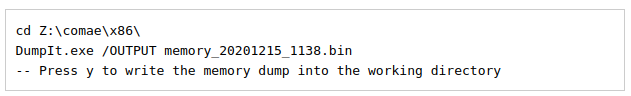
\includegraphics[scale=0.55]{images/dumpCmd.png}
                    \item[]
            \end{itemize} 
    \end{itemize}
    % 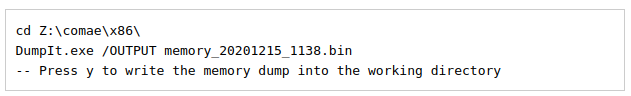
\includegraphics[scale=0.55]{images/dumpCmd.png}
\end{frame}


\begin{frame}
  \frametitle{7.2 Capturing memory}
      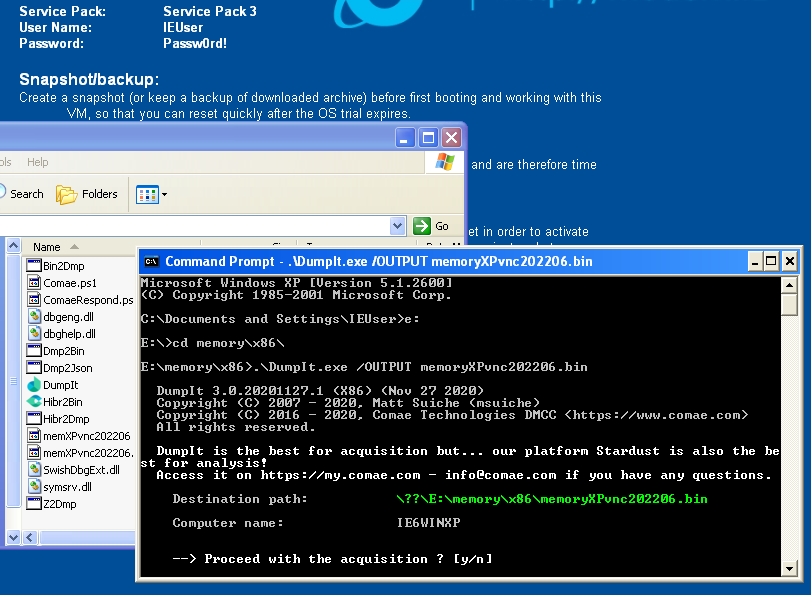
\includegraphics[scale=0.36]{images/dumpIt.png}
\end{frame}


\begin{frame}
  \frametitle{7.2 Capturing memory}
    \begin{itemize}
        \item Hibernation file: \texttt{hiberfil.sys}
            \begin{itemize}
		    \item[] Created when going into hibernation mode
		    \item[] Fully fleded memory content
		    \item[] Compressed and slightly modified
		    \item[] Can be converted into raw memory dump
		    \item[] Force hibernation:
                    \begin{itemize}
		        \item[] \texttt{powercfg /h[ibernate] [on|off]}
		        \item[] \texttt{psshutdown -h}
                    \end{itemize}
            \end{itemize}
        \item[]
        \item Pagefile: \texttt{pagefile.sys}
        \item[]
	\item Swapfile: \texttt{swapfile.sys} (Windows 8)
        \item[]
	\item Crash dump: \texttt{memory.dmp} (Blue Screen)
        \item[]
    \end{itemize}
\end{frame}


\begin{frame}[fragile]
  \frametitle{7.3 BulkExtractor Exercise}
    \begin{lstlisting}[basicstyle=\tiny]
1. Preparation
--------------

    sudo mount -o ro,offset=$((512*2048)) circl-dfir.dd /media/case1

    mkdir memory
    mkdir memory/out

    cp /media/case1/memory/* memory
    cd memory


2. BulkExtractor
----------------

    bulk_extractor -o out/ DEMO-PC-20180315-160249.raw


3. Investigate results
----------------------

    ls -lh out/

    less out/url_histogram.txt
    less out/email_histogram.txt
    less out/aes_keys.txt
    \end{lstlisting}
\end{frame}


\begin{frame}[fragile]
  \frametitle{7.4 Volatility Overview}
    \begin{itemize}
        \item[] Volatility 2 or Volatility 3
    \end{itemize}
    \begin{lstlisting}[basicstyle=\tiny]
python vol.py -h | less
python vol.py -info | less

     ...
     imagecopy      	Copies a physical address space out as a raw DD image
     imageinfo      	Identify information for the image
     ...
     pslist         	Print all running processes by following the EPROCESS lists 
     psscan         	Scan Physical memory for _EPROCESS pool allocations
     pstree         	Print process list as a tree
     psxview        	Find hidden processes with various process listings
     ...
     sockets        	Print list of open sockets
     sockscan       	Scan Physical memory for _ADDRESS_OBJECT objects (tcp sockets)
     ...


vol.py -f <filename> <plugin [options]> --profile=<profile>
vol.py -f memdump.raw imageinfo


sudo apt install python3-pefile
git clone https://github.com/volatilityfoundation/volatility3.git
    \end{lstlisting}
\end{frame}


\begin{frame}[fragile]
  \frametitle{7.4 Volatility Overview: Exercise}
    \begin{itemize}
        \item[] Identify profile:
    \end{itemize}
    \begin{lstlisting}[basicstyle=\tiny]
vol.py -f DEMO-PC-20180315-160249.raw imageinfo

      Suggested Profile(s) : Win7SP1x86_23418, Win7SP0x86, Win7SP1x86_24000, Win7SP1x86
                  AS Layer1 : IA32PagedMemory (Kernel AS)
                  AS Layer2 : FileAddressSpace (memory/DEMO-PC-20180315-160249.raw)
                   PAE type : No PAE
                        DTB : 0x185000L
                       KDBG : 0x82954c70L
       Number of Processors : 1
  Image Type (Service Pack) : 1
             KPCR for CPU 0 : 0x82955d00L
          KUSER_SHARED_DATA : 0xffdf0000L
        Image date and time : 2018-03-15 16:02:54 UTC+0000
  Image local date and time : 2018-03-15 17:02:54 +0100


    --> vol.py -f <filename> <plugin [options]> --profile=Win7SP1x86_23418


export VOLATILITY_PROFILE=Win7SP1x86_23418

    --> vol.py -f <filename> <plugin [options]> 
    \end{lstlisting}
\end{frame}


\begin{frame}[fragile]
  \frametitle{7.5 Volatility: Process Analysis}
    \begin{itemize}
        \item[] \texttt{pslist}
            \begin{itemize}
                \item Running processes
                \item Process IP - PID
                \item Parent PIP - PPID
                \item Start time
            \end{itemize}
        \item[] \texttt{pstree}
            \begin{itemize}
                \item Like \texttt{pslist}
                \item Visual child-parent relation
            \end{itemize}
        \item[] \texttt{psscan}
            \begin{itemize}
                \item Brute Force
                \item Find inactive and/or hidden processes
            \end{itemize}
        \item[] \texttt{psxview}
            \begin{itemize}
                \item Run and compare some tests
                \item Correlate \texttt{psscan} and \texttt{pslist}
            \end{itemize}
    \end{itemize}
\end{frame}


\begin{frame}[fragile]
  \frametitle{7.5 Volatility: Process Analysis}
    \begin{lstlisting}[basicstyle=\tiny]
volatility --profile=Win7SP1x86 -f Win-Enc-20190415.raw pslist > pslist.txt


  Offset(V)  Name             PID   PPID Thds  Hnds Ses Wow64 Start          
  ---------- ------------- ------ ------ ---- ----- --- -------------------------
  0x84233af0 System             4      0   70   505 ---    0 2019-04-15 15:02:52 UTC+0000 
  0x848d8288 smss.exe         248      4    2    29 ---    0 2019-04-15 15:02:52 UTC+0000
  0x8487a700 csrss.exe        324    308    9   384   0    0 2019-04-15 15:02:54 UTC+0000
  0x84fbb530 csrss.exe        360    352    7   274   1    0 2019-04-15 15:02:54 UTC+0000
  0x84fc3530 wininit.exe      368    308    3    77   0    0 2019-04-15 15:02:54 UTC+0000
  0x84fd0530 winlogon.exe     396    352    4   112   1    0 2019-04-15 15:02:54 UTC+0000
  0x85048a18 services.exe     456    368    8   203   0    0 2019-04-15 15:02:55 UTC+0000
  0x8505ac00 lsass.exe        464    368    7   580   0    0 2019-04-15 15:02:55 UTC+0000
  0x8505caa0 lsm.exe          472    368   10   145   0    0 2019-04-15 15:02:55 UTC+0000
  ...
  ...
  ...
  0x85050b60 WmiPrvSE.exe    3268    564    9   175   0    0 2019-04-15 15:06:52 UTC+0000
  0x8438bd40 owxxb-a.exe     3432   3368   15   471   1    0 2019-04-15 15:07:13 UTC+0000
  0x84394030 VSSVC.exe       3676    456    6   123   0    0 2019-04-15 15:07:22 UTC+0000
  0x84394488 svchost.exe     3728    456    6    70   0    0 2019-04-15 15:07:23 UTC+0000
  0x84a243c8 notepad.exe     3820   3432    1    64   1    0 2019-04-15 15:08:05 UTC+0000
  0x846d8030 iexplore.exe    3832   3432   19   427   1    0 2019-04-15 15:08:06 UTC+0000
  0x846d2d40 iexplore.exe    3908   3832   11   293   1    0 2019-04-15 15:08:07 UTC+0000
  0x846e5a58 dllhost.exe     3928    564    6    94   1    0 2019-04-15 15:08:07 UTC+0000
  0x84684d40 dllhost.exe     4012    564   10   212   1    0 2019-04-15 15:08:08 UTC+0000
    \end{lstlisting}
\end{frame}


\begin{frame}[fragile]
  \frametitle{7.5 Volatility: Process Analysis}
    \begin{lstlisting}[basicstyle=\tiny]
volatility --profile=Win7SP1x86 -f Win-Enc-20190415.raw psxview > psxview


  Offset(P)  Name          PID pslist psscan thrdproc pspcid csrss session deskthrd
  ---------- ---------- ------ ------ ------ -------- ------ ----- ------- --------
  .....
  .....
  0x3f60f030 taskhost.exe     352 True   True   True     True   True  True    True
  0x3fa84d40 dllhost.exe     4012 True   True   True     True   True  True    True
  0x3ec23148 spoolsv.exe     1296 True   True   True     True   True  True    True
  0x3f63f470 explorer.exe     920 True   True   True     True   True  True    True
  0x3ff0bd40 owxxb-a.exe     3432 True   True   True     True   True  True    True
  0x3f3d0530 winlogon.exe     396 True   True   True     True   True  True    True
  0x3f3c3530 wininit.exe      368 True   True   True     True   True  True    True
  0x3ec9f030 svchost.exe      688 True   True   True     True   True  True    True
  0x3ef3d758 VBoxTray.exe    1832 True   True   True     True   True  True    True
  0x3fae5a58 dllhost.exe     3928 True   True   True     True   True  True    True
  0x3ec50b60 WmiPrvSE.exe    3268 True   True   True     True   True  True    True
  0x3ec88b90 svchost.exe      564 True   True   True     True   True  True    True
  0x3ecd3768 svchost.exe      820 True   True   True     True   True  True    True
  0x3ef4f030 SearchIndexer.  2008 True   True   True     True   True  True    True
  0x3ec08d40 svchost.exe     1444 True   True   True     True   True  True    True
  0x3ed10d40 svchost.exe     1008 True   True   True     True   True  True    True
  0x3f6243c8 notepad.exe     3820 True   True   True     True   True  True    True
  0x3ecd95f8 svchost.exe      852 True   True   True     True   True  True    True
  0x3fad2d40 iexplore.exe    3908 True   True   True     True   True  True    True
  .....
  .....
    \end{lstlisting}
\end{frame}


\begin{frame}[fragile]
  \frametitle{7.6 Volatility: Network Analysis}
    \begin{itemize}
        \item Windows XP and 2003 Server
            \begin{itemize}
                \item \texttt{connections}
                \item \texttt{connscan}
                \item \texttt{sockets}
            \end{itemize}
        \item Windwos 7
            \begin{itemize}
                \item \texttt{netscan}
            \end{itemize}
    \end{itemize}
    \begin{lstlisting}[basicstyle=\tiny]
volatility --profile=Win7SP1x86 -f Win-Enc-20190415.raw netscan > netscan.txt


  Proto   Local Address       Foreign Address     State           Pid     Owner
  .....
  UDPv4   0.0.0.0:0           *:*                                2748     powershell.exe 
  UDPv6   :::0                *:*                                2748     powershell.exe
  TCPv4   0.0.0.0:49155       0.0.0.0:0           LISTENING       456     services.exe
  TCPv4   0.0.0.0:49156       0.0.0.0:0           LISTENING       464     lsass.exe
  TCPv6   :::49156            :::0                LISTENING       464     lsass.exe
  TCPv4   10.0.2.15:49167     2.17.201.11:80      ESTABLISHED    1128     svchost.exe
  TCPv4   10.0.2.15:49166     93.184.220.29:80    ESTABLISHED    1128     svchost.exe
  TCPv4   10.0.2.15:49165     50.62.124.1:80      ESTABLISHED    3432     owxxb-a.exe
  TCPv4   10.0.2.15:49160     216.239.32.21:80    ESTABLISHED    3432     owxxb-a.exe
  TCPv4   10.0.2.15:49162     2.17.201.8:80       ESTABLISHED    3432     owxxb-a.exe
  TCPv4   10.0.2.15:49168     13.107.21.200:80    ESTABLISHED    3832     iexplore.exe
  TCPv4   10.0.2.15:49159     94.23.7.52:80       CLOSE_WAIT     2748     powershell.exe
  .....
    \end{lstlisting}
\end{frame}


\begin{frame}[fragile]
  \frametitle{7.7 Volatility: Other plugins}
    \begin{itemize}
        \item Other useful plugins
    \begin{lstlisting}[basicstyle=\tiny]
volatility -f memdump.raw sessions
volatility -f memdump.raw privs
volatility -f memdump.raw hivelist
volatility -f memdump.raw filescan
volatility -f memdump.raw timeline
volatility -f memdump.raw hashdump
    \end{lstlisting}
        \item Get SIDs
    \begin{lstlisting}[basicstyle=\tiny]
volatility --profile=Win7SP1x86 -f Win-Enc-20190415.raw getsids

  powershell.exe (2748): S-1-5-21-3408732720-2018246097-660081352-1000 (John)
  owxxb-a.exe (3432): S-1-5-21-3408732720-2018246097-660081352-1000 (John)
  notepad.exe (3820): S-1-5-21-3408732720-2018246097-660081352-1000 (John)
  iexplore.exe (3832): S-1-5-21-3408732720-2018246097-660081352-1000 (John)
  iexplore.exe (3908): S-1-5-21-3408732720-2018246097-660081352-1000 (John)
  dllhost.exe (3928): S-1-5-21-3408732720-2018246097-660081352-1000 (John)
    \end{lstlisting}
    \end{itemize}
\end{frame}


\begin{frame}[fragile]
  \frametitle{7.7 Volatility: Other plugins}
    \begin{itemize}
        \item Command line history
    \begin{lstlisting}[basicstyle=\tiny]
vol.py --profile=Win7SP1x86 -f memdump.raw cmdline
vol.py --profile=Win7SP1x86 -f memdump.raw cmdscan
vol.py --profile=Win7SP1x86 -f memdump.raw consoles
    \end{lstlisting}
        \item Find suspicious processes
    \begin{lstlisting}[basicstyle=\tiny]
volatility --profile=Win7SP1x86 -f Win-Enc-20190415.raw malfind

  Process: owxxb-a.exe Pid: 3432 Address: 0x400000
  Vad Tag: VadS Protection: PAGE_EXECUTE_READWRITE
  Flags: CommitCharge: 134, MemCommit: 1, PrivateMemory: 1, Protection: 6

  0x00400000  4d 5a 90 00 03 00 00 00 04 00 00 00 ff ff 00 00   MZ..............
  0x00400010  b8 00 00 00 00 00 00 00 40 00 00 00 00 00 00 00   ........@.......
  0x00400020  00 00 00 00 00 00 00 00 00 00 00 00 00 00 00 00   ................
  0x00400030  00 00 00 00 00 00 00 00 00 00 00 00 08 01 00 00   ................

  0x00400000 4d               DEC EBP
  0x00400001 5a               POP EDX
  0x00400002 90               NOP
    \end{lstlisting}
    \end{itemize}
\end{frame}


\begin{frame}[fragile]
  \frametitle{7.8 Volatility Exercise}
    \begin{lstlisting}[basicstyle=\tiny]
python volatility3/vol.py -q --help | less
mkdir out2


python volatility3/vol.py -q -f ./DEMO-PC-20180315-160249.raw windows.pslist >out2/pslist
python volatility3/vol.py -q -f ./DEMO-PC-20180315-160249.raw windows.pstree >out2/pstree
python volatility3/vol.py -q -f ./DEMO-PC-20180315-160249.raw windows.psscan >out2/psscan
python volatility3/vol.py -q -f ./DEMO-PC-20180315-160249.raw windows.psxview >out2/psxview


python volatility3/vol.py -q -f ./DEMO-PC-20180315-160249.raw windows.netscan.NetScan >out2/NetSca


python volatility3/vol.py -q -f ./DEMO-PC-20180315-160249.raw windows.dumpfiles.DumpFiles >out2/DumpFiles
python volatility3/vol.py -q -f ./DEMO-PC-20180315-160249.raw windows.filescan.FileScan > out2/FileScan


python volatility3/vol.py -q -f ./DEMO-PC-20180315-160249.raw timeliner > out2/timeliner


python volatility3/vol.py -q -f ./DEMO-PC-20180315-160249.raw windows.registry.hivelist.HiveList > out2/hivelist


python volatility3/vol.py -q -f ./DEMO-PC-20180315-160249.raw windows.consoles.Consoles > out2/consoles
python volatility3/vol.py -q -f ./DEMO-PC-20180315-160249.raw windows.cmdline.CmdLine > out2/cmdline
python volatility3/vol.py -q -f ./DEMO-PC-20180315-160249.raw windows.cmdline.CmdScan > out2/cmdscan
    \end{lstlisting}
\end{frame}








\include{f39_out}


\begin{frame}
  \frametitle{Overview}
  \begin{itemize}
  \item[]
      \begin{enumerate}
%          \setcounter{enumi}{10}
          \item Windows Registry
          \item Event Logs
          \item Other Sources of Information
          \item Malware Analysis
          \item Analysing files
          \item Live Response
          \item Memory Forensics
          \item Bibliography and Outlook
      \end{enumerate}

  \end{itemize}
\end{frame}


\end{document}

